\documentclass[11pt,a4paper]{article}
\usepackage[margin=22mm]{geometry}
\usepackage{amsmath,amssymb,booktabs,tabularx,array,graphicx,xcolor,fancyhdr,hyperref,float}
\usepackage[american]{circuitikz}
\usepackage{caption}
\hypersetup{colorlinks=true,linkcolor=black,urlcolor=blue,citecolor=black,pdftitle={Analysis and LTspice Simulation of a Triple Voltage-Lift Modified Luo Converter},pdfauthor={Aly Hany Rakha}}
\definecolor{navy}{RGB}{32,65,90}
\setlength{\parindent}{0pt}\setlength{\parskip}{6pt}
\renewcommand{\arraystretch}{1.18}
\pagestyle{fancy}\fancyhf{}\fancyhead[L]{\small Aly Hany Rakha}\fancyhead[R]{\small CO-526 | Paper P08}\fancyfoot[C]{\thepage}
\setlength{\headheight}{14pt}\setlength{\emergencystretch}{2em}
\captionsetup{font=small,labelfont=bf}
\newcommand{\unit}[1]{\,\mathrm{#1}}
\newcommand{\fig}[3]{\begin{figure}[H]\centering\includegraphics[width=#2\linewidth]{figures/#1}\caption{#3}\end{figure}}
\begin{document}
\begin{center}
{\Large\bfseries Analysis and LTspice Simulation of a Triple Voltage-Lift Modified Luo Converter}\par
\vspace{4mm}
{\large Aly Hany Rakha}\par
CO-526 Electronics Laboratory\quad |\quad IEEE Paper P08\par
28 October 2026
\end{center}
\vspace{2mm}
\begin{abstract}
This report examines the modified Luo converters proposed by Gholizadeh et al. and reproduces the triple voltage-lift circuit in LTspice. The analysis follows the two switching states, derives the voltage gain and capacitor voltages, and compares these predictions with transient simulations. With a 50 V input, 100 kHz switching frequency and approximately 50\% duty cycle, the near-ideal model gives an average output of 299.45 V, compared with the ideal prediction of 300 V. Both inductor currents remain positive in the measured steady-state interval. Tests at 30\% and 60\% duty give 213.97 V and 374.41 V, respectively. Additional models introduce conduction losses and replace the ideal switch with a MOSFET model. The final MOSFET simulation gives 295.10 V and a simulated efficiency of 97.58\%, including the gate source power. These results support the steady-state operating principle, while the startup overshoot, model simplifications and sensitivity of small ripple measurements limit what can be concluded about hardware performance.
\end{abstract}
\section{Purpose and scope}
Renewable energy sources often provide a DC voltage below the level required by the next conversion stage. A step-up converter raises that voltage by storing energy and transferring it to the output through a controlled switching process. For an ordinary boost converter, a large voltage ratio requires a high duty cycle. This reduces the available off-time and can increase practical losses and device demands.

The selected paper proposes triple, quadruple and hextuple voltage-lift modified Luo converters \cite{paper}. Their central idea is to combine inductors with a network of capacitors and diodes so that stored capacitor voltages contribute to the output. All three versions use one controlled switch and two inductors, with a common input and output ground.

I focused the simulation on the triple converter. This allows the circuit operation to be checked in detail before considering the larger extensions. The work includes the circuit schematic, startup response, steady-state voltages and currents, a duty-cycle comparison, and progressively less ideal device models. The quadruple and hextuple circuits are discussed from the paper; they were not simulated in this work. No physical prototype was built.

\textbf{Reference operating point.} The abstract of the paper describes a 150 W prototype, whereas its experimental section describes a 100 W prototype. Tables I and II specify approximately 300 V and 0.33 A, which correspond to 99 W. I therefore use the tabulated approximately 100 W operating point as the reference for this replication. This distinction matters when comparing the load, current and power results.
\clearpage
\section{Circuit structure and the purpose of each component}
Figure~\ref{fig:circuit} shows the triple converter used for the analysis. The capacitors are not all connected across ground: in particular, $C_1$, $C_3$ and $C_5$ must be measured between their own terminals. A voltage measured from one of these terminals to ground is not necessarily the voltage across that capacitor.
\begin{figure}[H]\centering
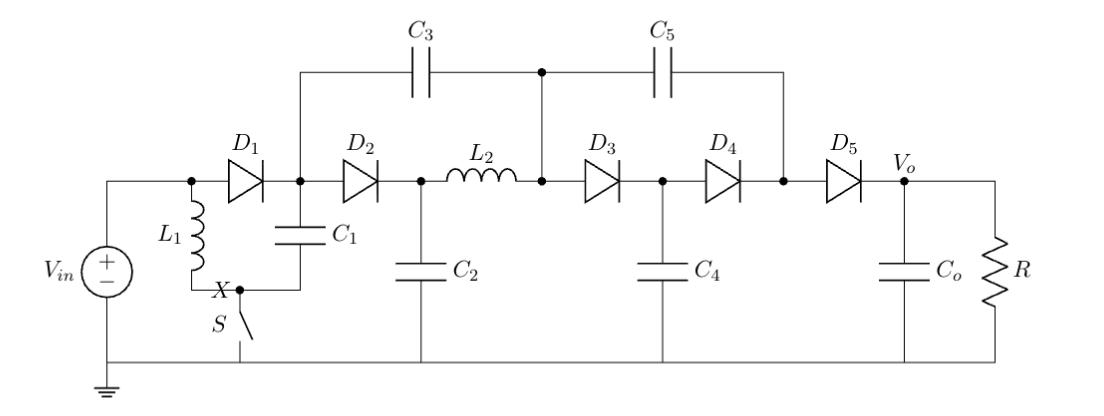
\includegraphics[width=\linewidth]{figures/circuit_supplied.png}
\caption{Triple voltage-lift power circuit. Topology reproduced from Gholizadeh et al. \cite{paper}; the image was supplied with the project materials and shows the same power-stage connections as the simulation. $S$ is the controlled switch; its pulse source is omitted here for clarity.}\label{fig:circuit}
\end{figure}
\begin{tabularx}{\linewidth}{@{}lX@{}}\toprule
Component & Function in the conversion process \\\midrule
$V_{in}$ & Supplies 50 V DC to both the $L_1$ branch and the diode network. \\\
$L_1$ & Stores energy while the switch is on and maintains current during the off interval. Its voltage balance helps set the lifted capacitor voltages. \\\
$L_2$ & Stores and transfers energy in the second conversion path; its average current equals the load current in ideal steady-state operation. \\\
$C_1$ & Charges to approximately the input voltage and provides the first voltage-lift contribution. \\\
$C_2$ & Provides an intermediate energy reservoir and supplies the $L_2$ charging path during the on interval. \\\
$C_3$ & Connects two floating circuit nodes and supplies a duty-dependent voltage-lift contribution. \\\
$C_4$ & Holds the intermediate voltage before the final lift stage. \\\
$C_5$ & Adds its voltage to $C_4$ during output energy transfer. \\\
$C_o$ & Supplies the load while $D_5$ is blocked and reduces output ripple. \\\
$D_1$--$D_5$ & Select the charging and discharging paths as node voltages change. They do not require separate control signals. \\\
$S$ and drive & Alternate the two circuit states. The duty cycle controls the ideal conversion ratio. \\\
$R$ & Represents a resistive load; $909.09\unit{\Omega}$ gives approximately 0.33 A at 300 V. \\\bottomrule
\end{tabularx}

For the equations below, $V_{C1}$ is positive at the top of $C_1$, and $V_{C3}$ and $V_{C5}$ are positive at their right-hand terminals in Figure~\ref{fig:circuit}. The other capacitor voltages are positive at their upper terminals. These choices match the measurement expressions used in LTspice.
\clearpage
\section{How the converter operates}
The starting point is that an inductor current cannot change instantaneously, and a capacitor voltage cannot change instantaneously in the ideal finite-current model. When the switch changes state, these stored quantities force the diode network into a different conduction pattern. The following explanation assumes continuous conduction mode (CCM), ideal devices and approximately constant capacitor voltages within one switching period.
\subsection{Switch on: energy storage and capacitor charging}
When $S$ closes, node $X$ is brought close to ground. Diodes $D_1$ and $D_4$ conduct, while $D_2$, $D_3$ and $D_5$ block. The input applies a positive voltage across $L_1$, causing its current to rise. Through $D_1$, $C_1$ is charged to approximately $V_{in}$.

The voltage across $L_2$ is set by $C_2$, $C_3$ and the clamped $C_1$ voltage. Its current also rises at the reference operating point. The $D_4$ path connects the $C_4$ reservoir to the lift-capacitor network. Because $D_5$ is blocked, the output is separated from this charging network, and $C_o$ supplies the load during this interval.

With inductor voltages defined in the direction of positive current, the on-state relations are
\begin{align}
 v_{L1,on}&=V_{in}, & v_{L2,on}&=V_{C2}-V_{C3}-V_{in},\\
 V_{C1}&=V_{in}, & V_{C4}&=V_{C1}+V_{C3}+V_{C5}.
\end{align}
The positive inductor voltages increase the stored magnetic energy, $E_L=\tfrac12 Li_L^2$. The output capacitor loses some charge while feeding the load, so its voltage falls slightly.
\subsection{Switch off: energy transfer to the output}
When $S$ opens, the current in $L_1$ must continue. Node $X$ rises, and the diode pattern changes: $D_2$, $D_3$ and $D_5$ conduct, while $D_1$ and $D_4$ block. The first inductor transfers energy through the $C_1$ and $D_2$ path toward the intermediate reservoir. The second inductor transfers energy through the paths to $C_4$ and to the output via $C_5$ and $D_5$.

The output receives the sum of two capacitor voltages, rather than the input voltage alone. The corresponding relations are
\begin{align}
 v_{L1,off}&=2V_{in}-V_{C2}, & v_{L2,off}&=-V_{C3},\\
 V_{C3}&=V_{C4}-V_{C2}, & V_o&=V_{C4}+V_{C5}.
\end{align}
At steady state, the negative off-state inductor voltages reduce the currents by the same amount that they rose during the on interval. The currents therefore repeat every switching period rather than increasing indefinitely.
\subsection{What the switching waveforms should show}
The voltage across the switch is low when it conducts and high when it blocks. This explains why the drain-voltage waveform is approximately the inverse of the gate-drive waveform. The inductor currents should have rising and falling ramps. A positive minimum current confirms CCM for that measured interval; it does not imply that the entire startup transient is also in CCM.
\clearpage
\section{Steady-state predictions}
Let $D$ be the on-time fraction and $T_s=1/f_s$ the switching period. In periodic steady state, the average voltage across each inductor is zero. Applying this to $L_1$ gives
\begin{equation}
D V_{in}+(1-D)(2V_{in}-V_{C2})=0
\quad\Rightarrow\quad V_{C2}=\frac{2-D}{1-D}V_{in}.
\end{equation}
For $L_2$,
\begin{equation}
D(V_{C2}-V_{C3}-V_{in})-(1-D)V_{C3}=0
\quad\Rightarrow\quad V_{C3}=\frac{D}{1-D}V_{in}.
\end{equation}
Combining these results with the capacitor relations gives
\begin{align}
V_{C1}&=V_{in}, & V_{C4}&=\frac{2V_{in}}{1-D}, & V_{C5}&=\frac{V_{in}}{1-D},\\
\boxed{M=\frac{V_o}{V_{in}}=\frac{3}{1-D}}.&&&
\end{align}
At $V_{in}=50\unit{V}$ and $D=0.5$, the gain is six and the predicted output is 300 V. ``Triple voltage-lift'' therefore refers to the factor of three relative to the conventional boost gain, not a fixed output equal to three times the input.

During the off interval, the switch blocks approximately
\begin{equation}
V_{S,off}=V_{C2}-V_{C1}=\frac{V_{in}}{1-D}=\frac{V_o}{3}.
\end{equation}
This predicts 100 V at the reference point. It is a steady-state result, not a bound on startup overshoot. The paper also gives this ideal blocking-voltage level for the diodes. The present simulation explicitly measures switch voltage; individual diode stress was not separately tabulated.

Using the paper's ideal charge-balance results,
\begin{equation}
I_{L1}=\frac{2+D}{1-D}I_o,\qquad I_{L2}=I_o,\qquad I_o=\frac{V_o}{R}.
\end{equation}
This gives $I_{L1}\approx1.65\unit{A}$ and $I_{L2}\approx0.33\unit{A}$. Here, $I_{L1}$ is not the total input current: the input also feeds the $D_1$ branch. Input power must therefore be measured at the source.

For small ripple, the inductor on-state slopes and output-capacitor discharge give
\begin{equation}
\Delta i_{L1}\simeq\frac{D V_{in}}{L_1f_s},\qquad
\Delta i_{L2}\simeq\frac{D V_{in}}{L_2f_s},\qquad
\Delta V_o\simeq\frac{D I_o}{C_of_s}.
\end{equation}
At 50\% duty these predict 0.125 A peak-to-peak for both inductors and approximately 33 mV output ripple. These expressions neglect ESR, finite diode drops and switching transients.

\textbf{A point requiring care in the paper.} Equation (4) prints $(1-D)V_{in}/(L_2f_s)$ for the second inductor ripple. However, substituting the derived capacitor voltages into its on-state equation gives $v_{L2,on}=V_{in}$ and therefore $D V_{in}/(L_2f_s)$. The two expressions agree at 50\% duty, so the reference case alone cannot distinguish them. Section~\ref{sec:duty} tests this apparent inconsistency away from 50\% duty.
\clearpage
\section{LTspice implementation and measurement method}
The circuit was implemented in LTspice 26.0.2 for macOS. The simulation uses the paper's tabulated inductance, capacitance, switching frequency and input voltage. The load is chosen from $R=300/0.33=909.09\unit{\Omega}$. The input source, output capacitor, load and switch return share the same ground.
\begin{table}[H]\centering\caption{Common simulation settings.}
\begin{tabular}{@{}ll@{}}\toprule
Quantity & Setting \\\midrule
Input voltage & 50 V DC \\\
Inductors $L_1,L_2$ & 2 mH each \\\
Capacitors $C_1$--$C_5,C_o$ & $50\unit{\mu F}$ each \\\
Load & $909.09\unit{\Omega}$ \\\
Switching frequency / period & 100 kHz / $10\unit{\mu s}$ \\\
Gate or control pulse & 0--10 V, 10 ns rise and fall times \\\
Simulation duration & 400 ms, \texttt{startup} option \\\
Average and minimum measurements & 390--400 ms \\\
Peak-to-peak ripple measurements & 399.9--400 ms (10 periods) \\\
Usual maximum timestep & 100 ns \\\
Final MOSFET check & 50 ns; waveform compression disabled \\\bottomrule
\end{tabular}
\end{table}
The 50\% control waveform is entered as
\begin{center}\texttt{PULSE(0 10 0 10n 10n 4.99u 10u)}.\end{center}
The 30\% and 60\% cases use pulse widths of \texttt{2.99u} and \texttt{5.99u}. The finite edges account for the small difference between these entered widths and an exact fraction of the period. For the ideal switch with a 5 V threshold, the resulting conduction intervals are approximately 3, 5 and $6\unit{\mu s}$.

The first model is called \emph{near-ideal}, because it still contains finite resistance: switch and diode on-resistances are $10\unit{m\Omega}$, inductor series resistances are $1\unit{m\Omega}$, diode forward threshold is zero, and no capacitor ESR is explicitly added. The switch and diode off-resistances are $1\unit{G\Omega}$. Small resistances permit loss and help avoid a completely lossless network.

Later models add assumed conduction losses and a MOSFET, as described in Section~\ref{sec:loss}. This sequence separates validation of the conversion principle from the effect of more detailed device behavior. The assumed loss values are not presented as measured parameters from the paper's prototype.

The \texttt{startup} option affects the initial energization of sources; it is not a designed soft-start controller. The plotted startup overshoot therefore belongs to this particular open-loop simulation and its initial conditions.

Floating capacitor voltages were measured between their terminals: $C_1$: \texttt{V(n001,n008)}, $C_3$: \texttt{V(n002,n001)}, and $C_5$: \texttt{V(n003,n002)}. The output is \texttt{V(n007)}. Node numbers refer to the supplied netlists and should be rechecked if the schematic is rewired.

\clearpage
\subsection{Simulation schematic and reasoning behind the tests}
\begin{figure}[H]\centering
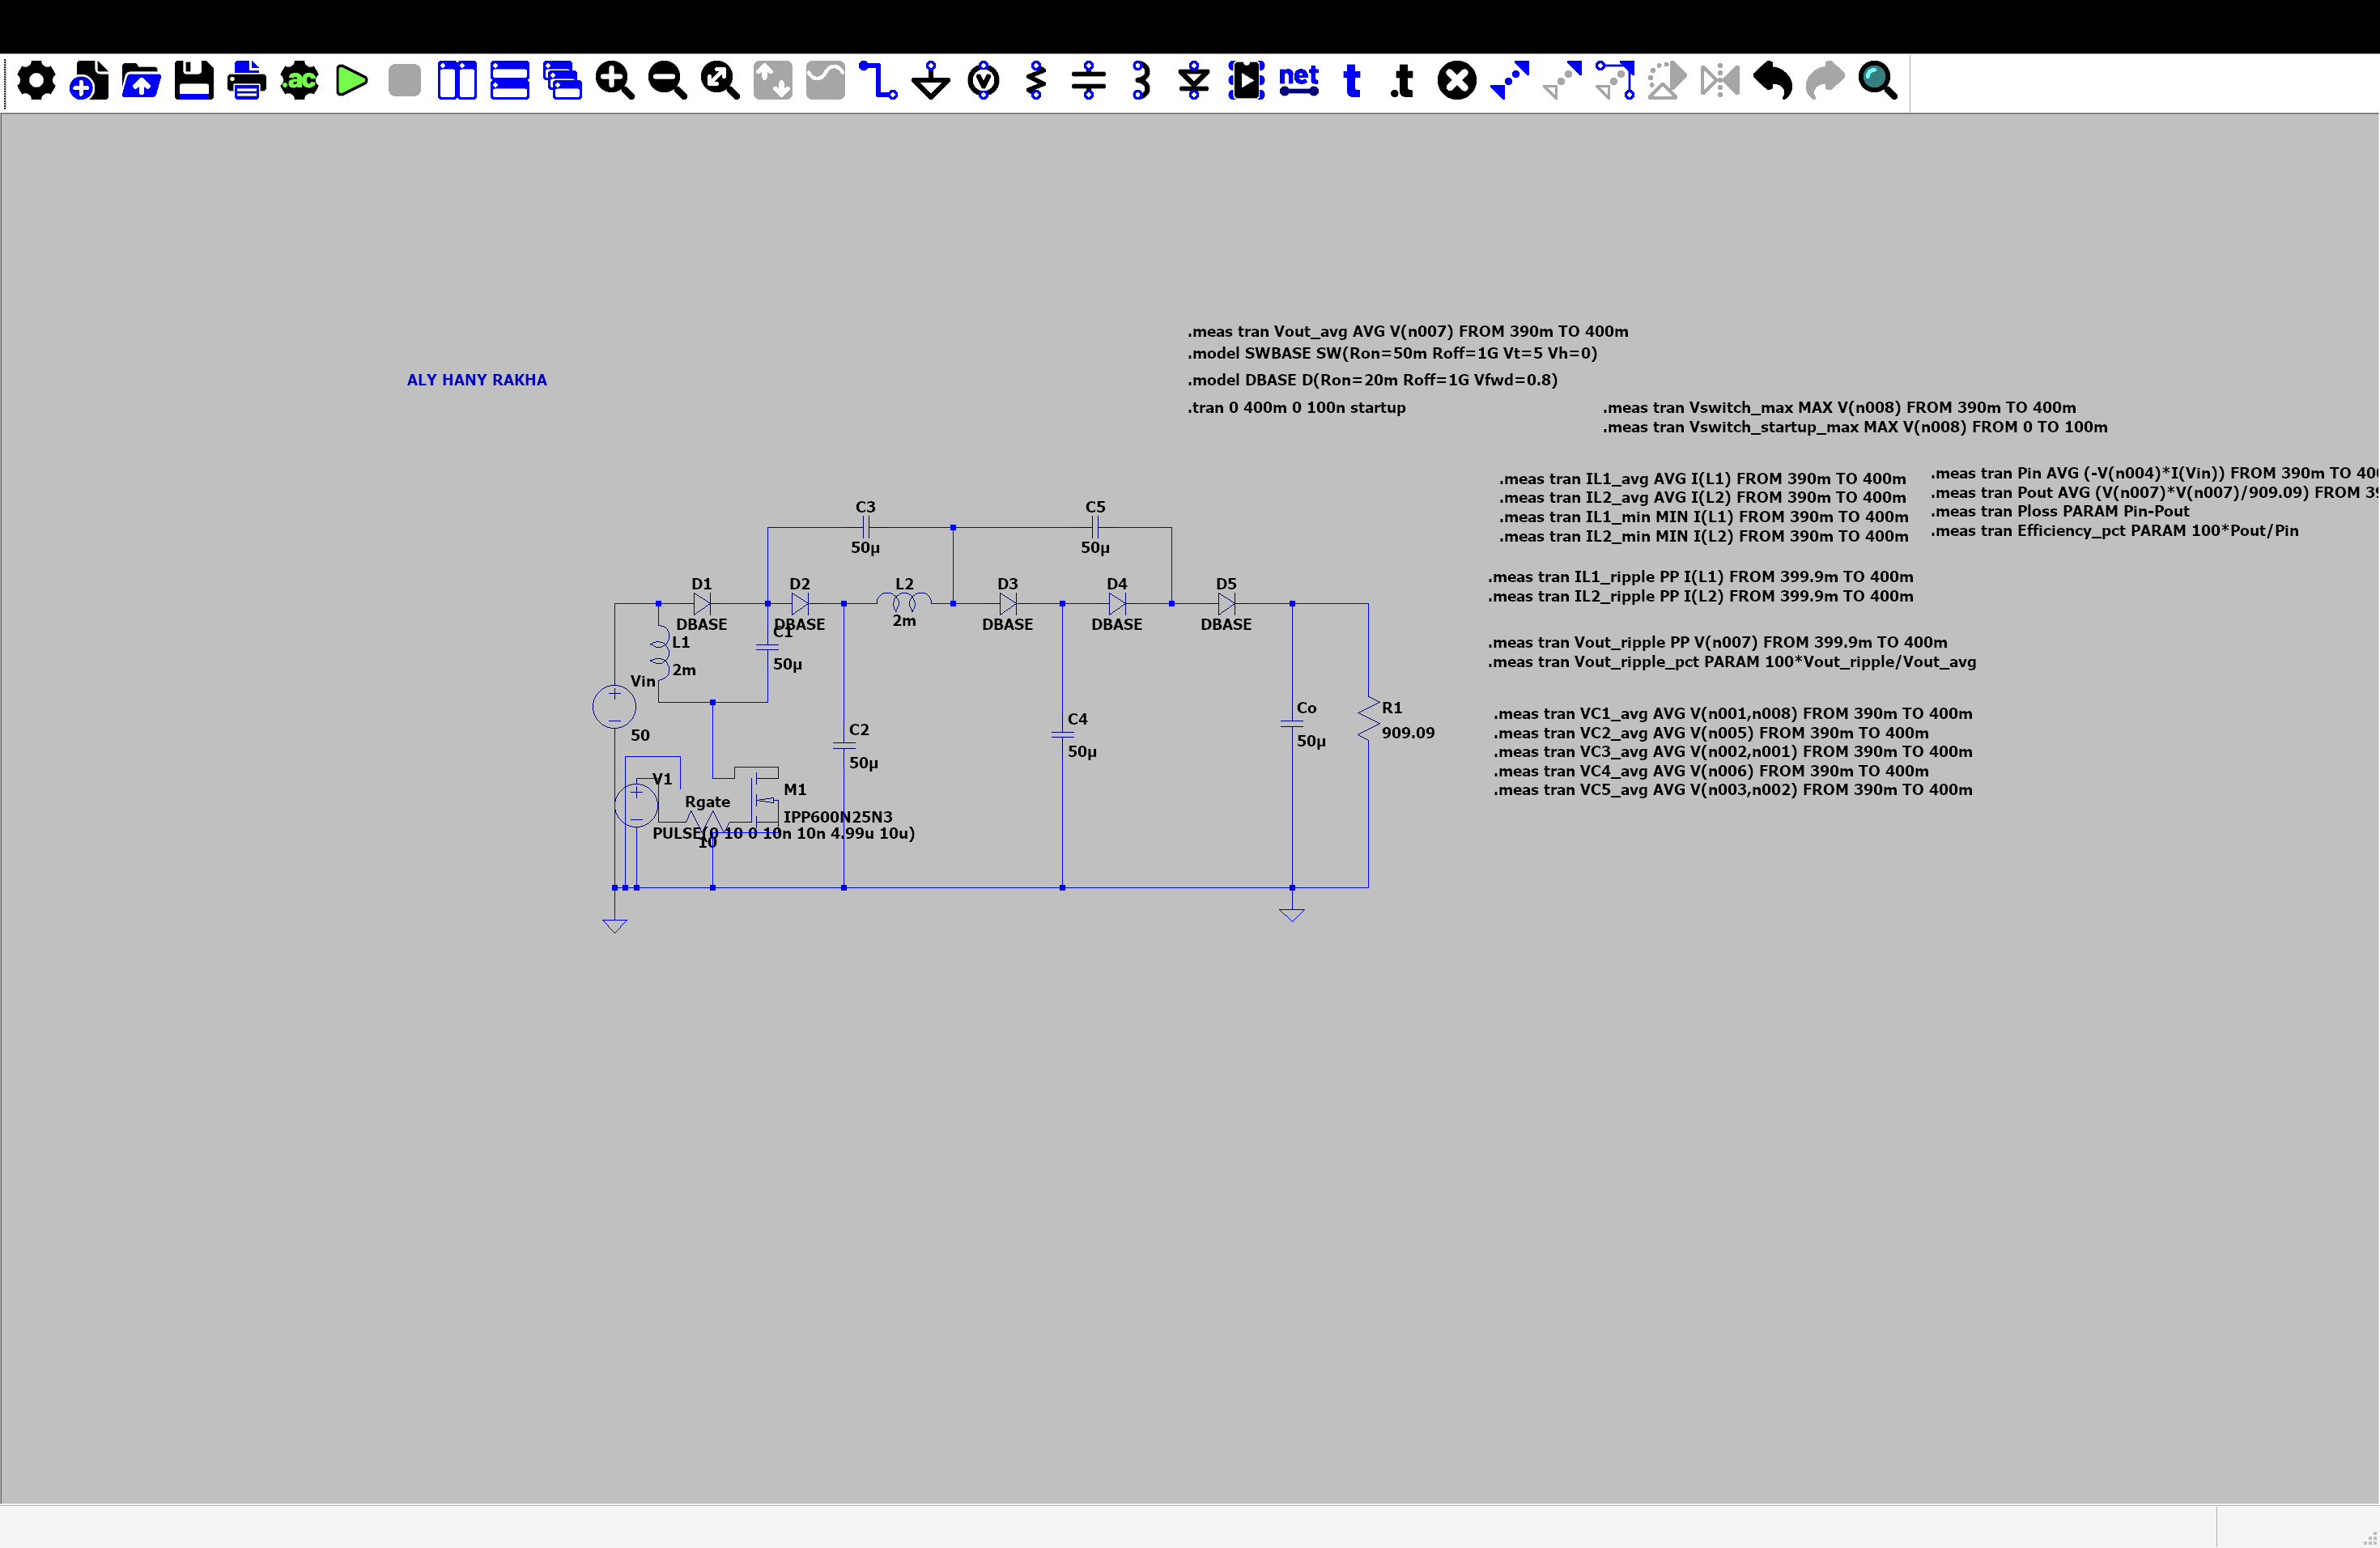
\includegraphics[trim={226bp 361bp 577bp 214bp},clip,width=\linewidth]{figures/photo25.png}
\caption{Original LTspice schematic capture, cropped to the power stage and author name, after replacing the controlled switch with a MOSFET and adding its gate resistor. The author's name is visible at the upper left. The final check uses the same power-stage connections with the numerical settings stated in Table 1.}\label{fig:ltcircuit}
\end{figure}
The schematic in Figure~\ref{fig:ltcircuit} connects the MOSFET drain to node $X$, its source to ground, and its gate to the pulse source through $R_{gate}$. The gate pulse controls the device; it is separate from the 50 V source that supplies the power stage. The diode arrows and capacitor connections follow the circuit in Figure~\ref{fig:circuit}. The small text in the screenshot is also available in the included schematics and netlists.

I started with the near-ideal switch so that the basic circuit could be compared directly with the equations. Matching only the output voltage would have been a weak check: a circuit can produce a plausible output while an intermediate connection is wrong. I therefore checked each capacitor voltage and both inductor currents before changing the device models.

The 30\% and 60\% tests then checked whether the same circuit followed the gain equation away from the reference point. Keeping the load resistance fixed made the test easy to interpret, but also changed the output power. Finally, the conduction-loss and MOSFET cases showed how the predictions changed when finite voltage drops, resistances and gate charging were included.

The debugging steps also affected how the measurements were made. A current trace initially looked flat because its vertical scale still included the large startup peak. Zooming to five settled periods and changing the current axes revealed the triangular ripple. For the loss model, an invalid \texttt{Rser} entry on the load resistor had to be removed: the load itself is already a resistance, while \texttt{Rser} was used to represent losses in the inductors and capacitors. These checks helped separate a plotting or setup problem from a problem with the converter.
\clearpage
\section{Baseline results at 50\% duty}
The output settles close to the predicted 300 V. Table~\ref{tab:base} compares the measured averages with the ideal analysis. The small reduction is consistent with using finite resistances instead of perfectly ideal components.
\begin{table}[H]\centering\caption{Near-ideal reference case, averaged over 390--400 ms.}\label{tab:base}
\begin{tabular}{@{}lrr@{}}\toprule
Quantity & Ideal prediction & LTspice \\\midrule
Output voltage (V) & 300.00 & 299.45 \\\
$V_{C1}$ (V) & 50.00 & 49.94 \\\
$V_{C2}$ (V) & 150.00 & 149.86 \\\
$V_{C3}$ (V) & 50.00 & 49.92 \\\
$V_{C4}$ (V) & 200.00 & 199.71 \\\
$V_{C5}$ (V) & 100.00 & 99.75 \\\
$I_{L1}$ (A) & 1.650 & 1.647 \\\
$I_{L2}$ (A) & 0.330 & 0.330 \\\bottomrule
\end{tabular}
\end{table}
The output differs from the ideal 300 V by $-0.183\%$. The capacitor results are especially useful because they test the intermediate lift stages, not just the final gain. For example, $V_{C4}+V_{C5}=299.46\unit{V}$ is very close to the measured output, with a small difference due to the conducting output diode and rounding.
\begin{figure}[H]\centering
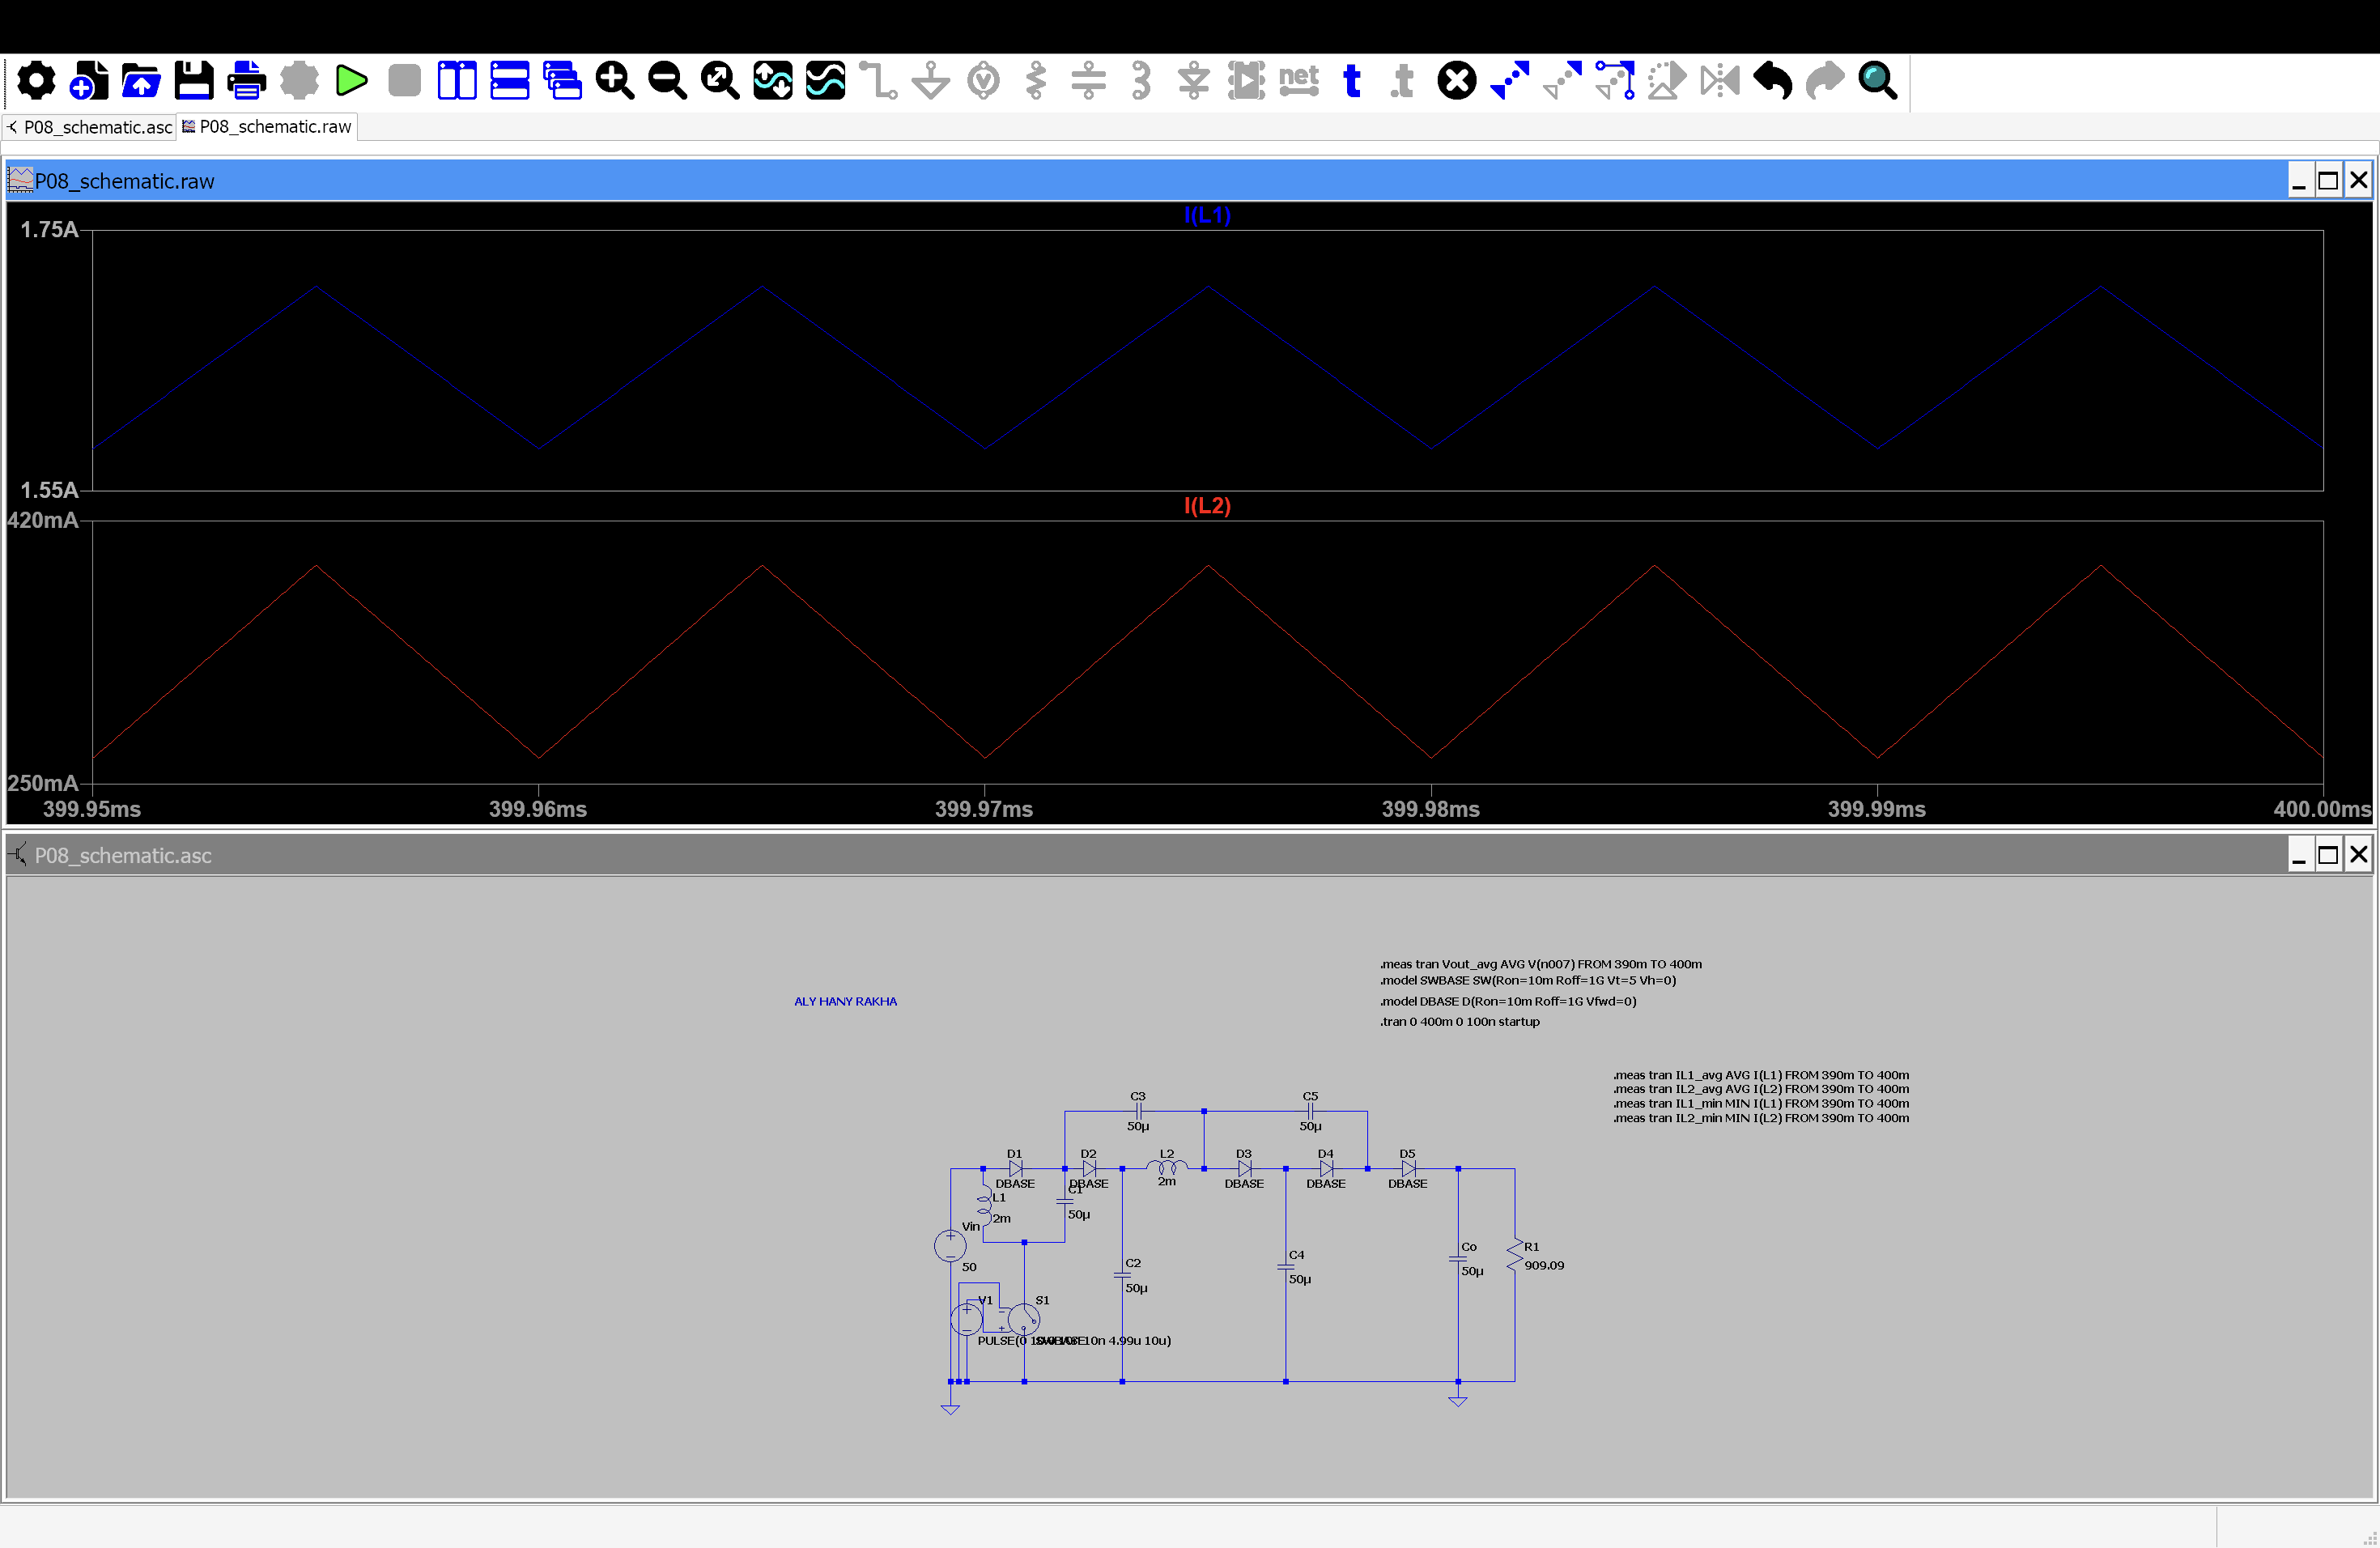
\includegraphics[trim={0bp 444bp 0bp 98bp},clip,width=1\linewidth]{figures/photo12.png}
\caption{Original LTspice screenshot of the settled inductor currents over five switching periods. The plot window is cropped from the full screenshot; traces, labels and axes are unchanged.}
\end{figure}
The minimum currents are 1.581 A for $L_1$ and 0.266 A for $L_2$, confirming CCM in the measured steady-state interval. Their peak-to-peak ripples are 0.12490 A and 0.12473 A, close to the 0.125 A prediction. The output ripple is 33.20 mV, or $0.01109\%$ of the average output.

The same absolute ripple represents about 7.6\% of the average $L_1$ current but 37.8\% of the average $L_2$ current. Thus the paper's stated 30\% current-ripple design target is not achieved for $L_2$ by the tabulated 2 mH value under this ripple definition, although its current remains continuous. Meeting that target would require approximately $2.53\unit{mH}$ from the ideal ripple estimate.
\clearpage
\subsection{Startup and switch voltage}
\begin{figure}[H]\centering
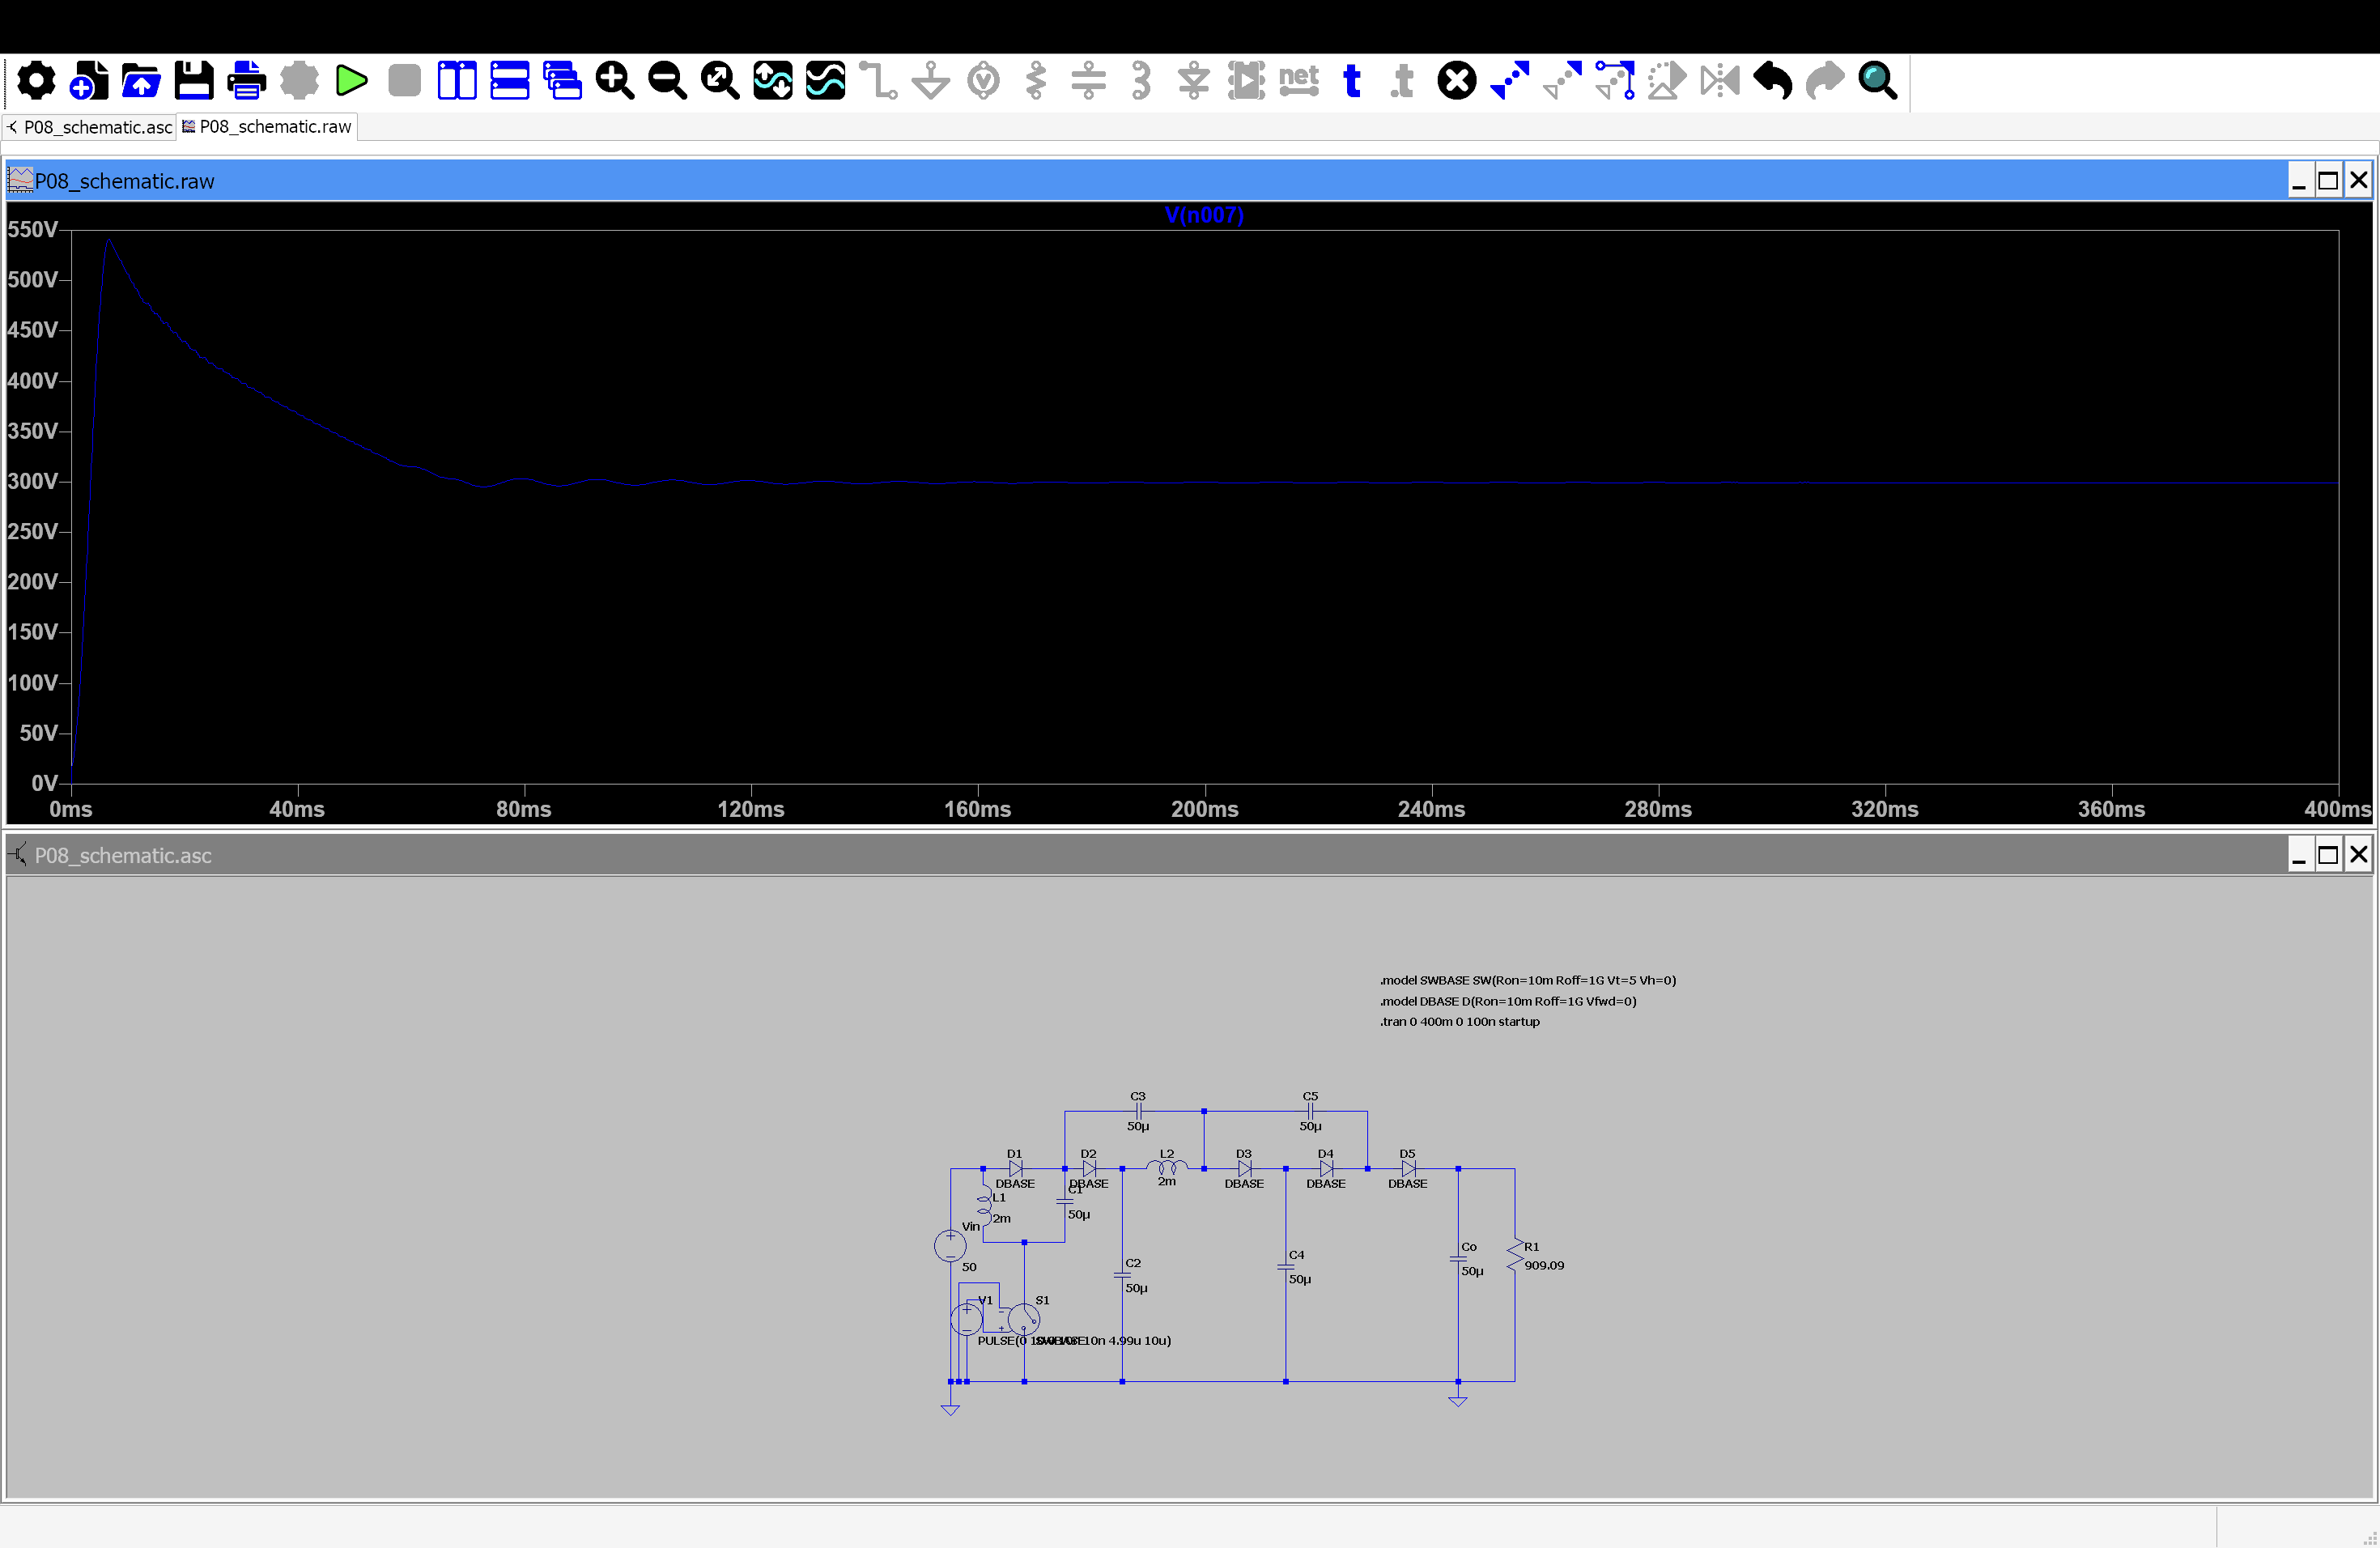
\includegraphics[trim={0bp 444bp 0bp 98bp},clip,width=1\linewidth]{figures/photo07.png}
\caption{Original LTspice output startup waveform. The screenshot is cropped to the plot window. The initial overshoot is much larger than the final ripple.}
\end{figure}
The output initially rises above its final value and then decays with damped oscillations. From the plotted trace, the output peak is approximately 540 V. This is a visual estimate, not a dedicated maximum measurement. Energy exchange between inductors and capacitors, combined with the small losses and abrupt open-loop energization, produces a pronounced transient.

The measured switch-voltage maximum is 100.07 V over 390--400 ms, agreeing with $V_{in}/(1-D)=100\unit{V}$. Over the first 100 ms, however, its maximum is 202.19 V. A component selected only from the steady-state expression would therefore miss the larger startup stress in this simulation.
\begin{figure}[H]\centering
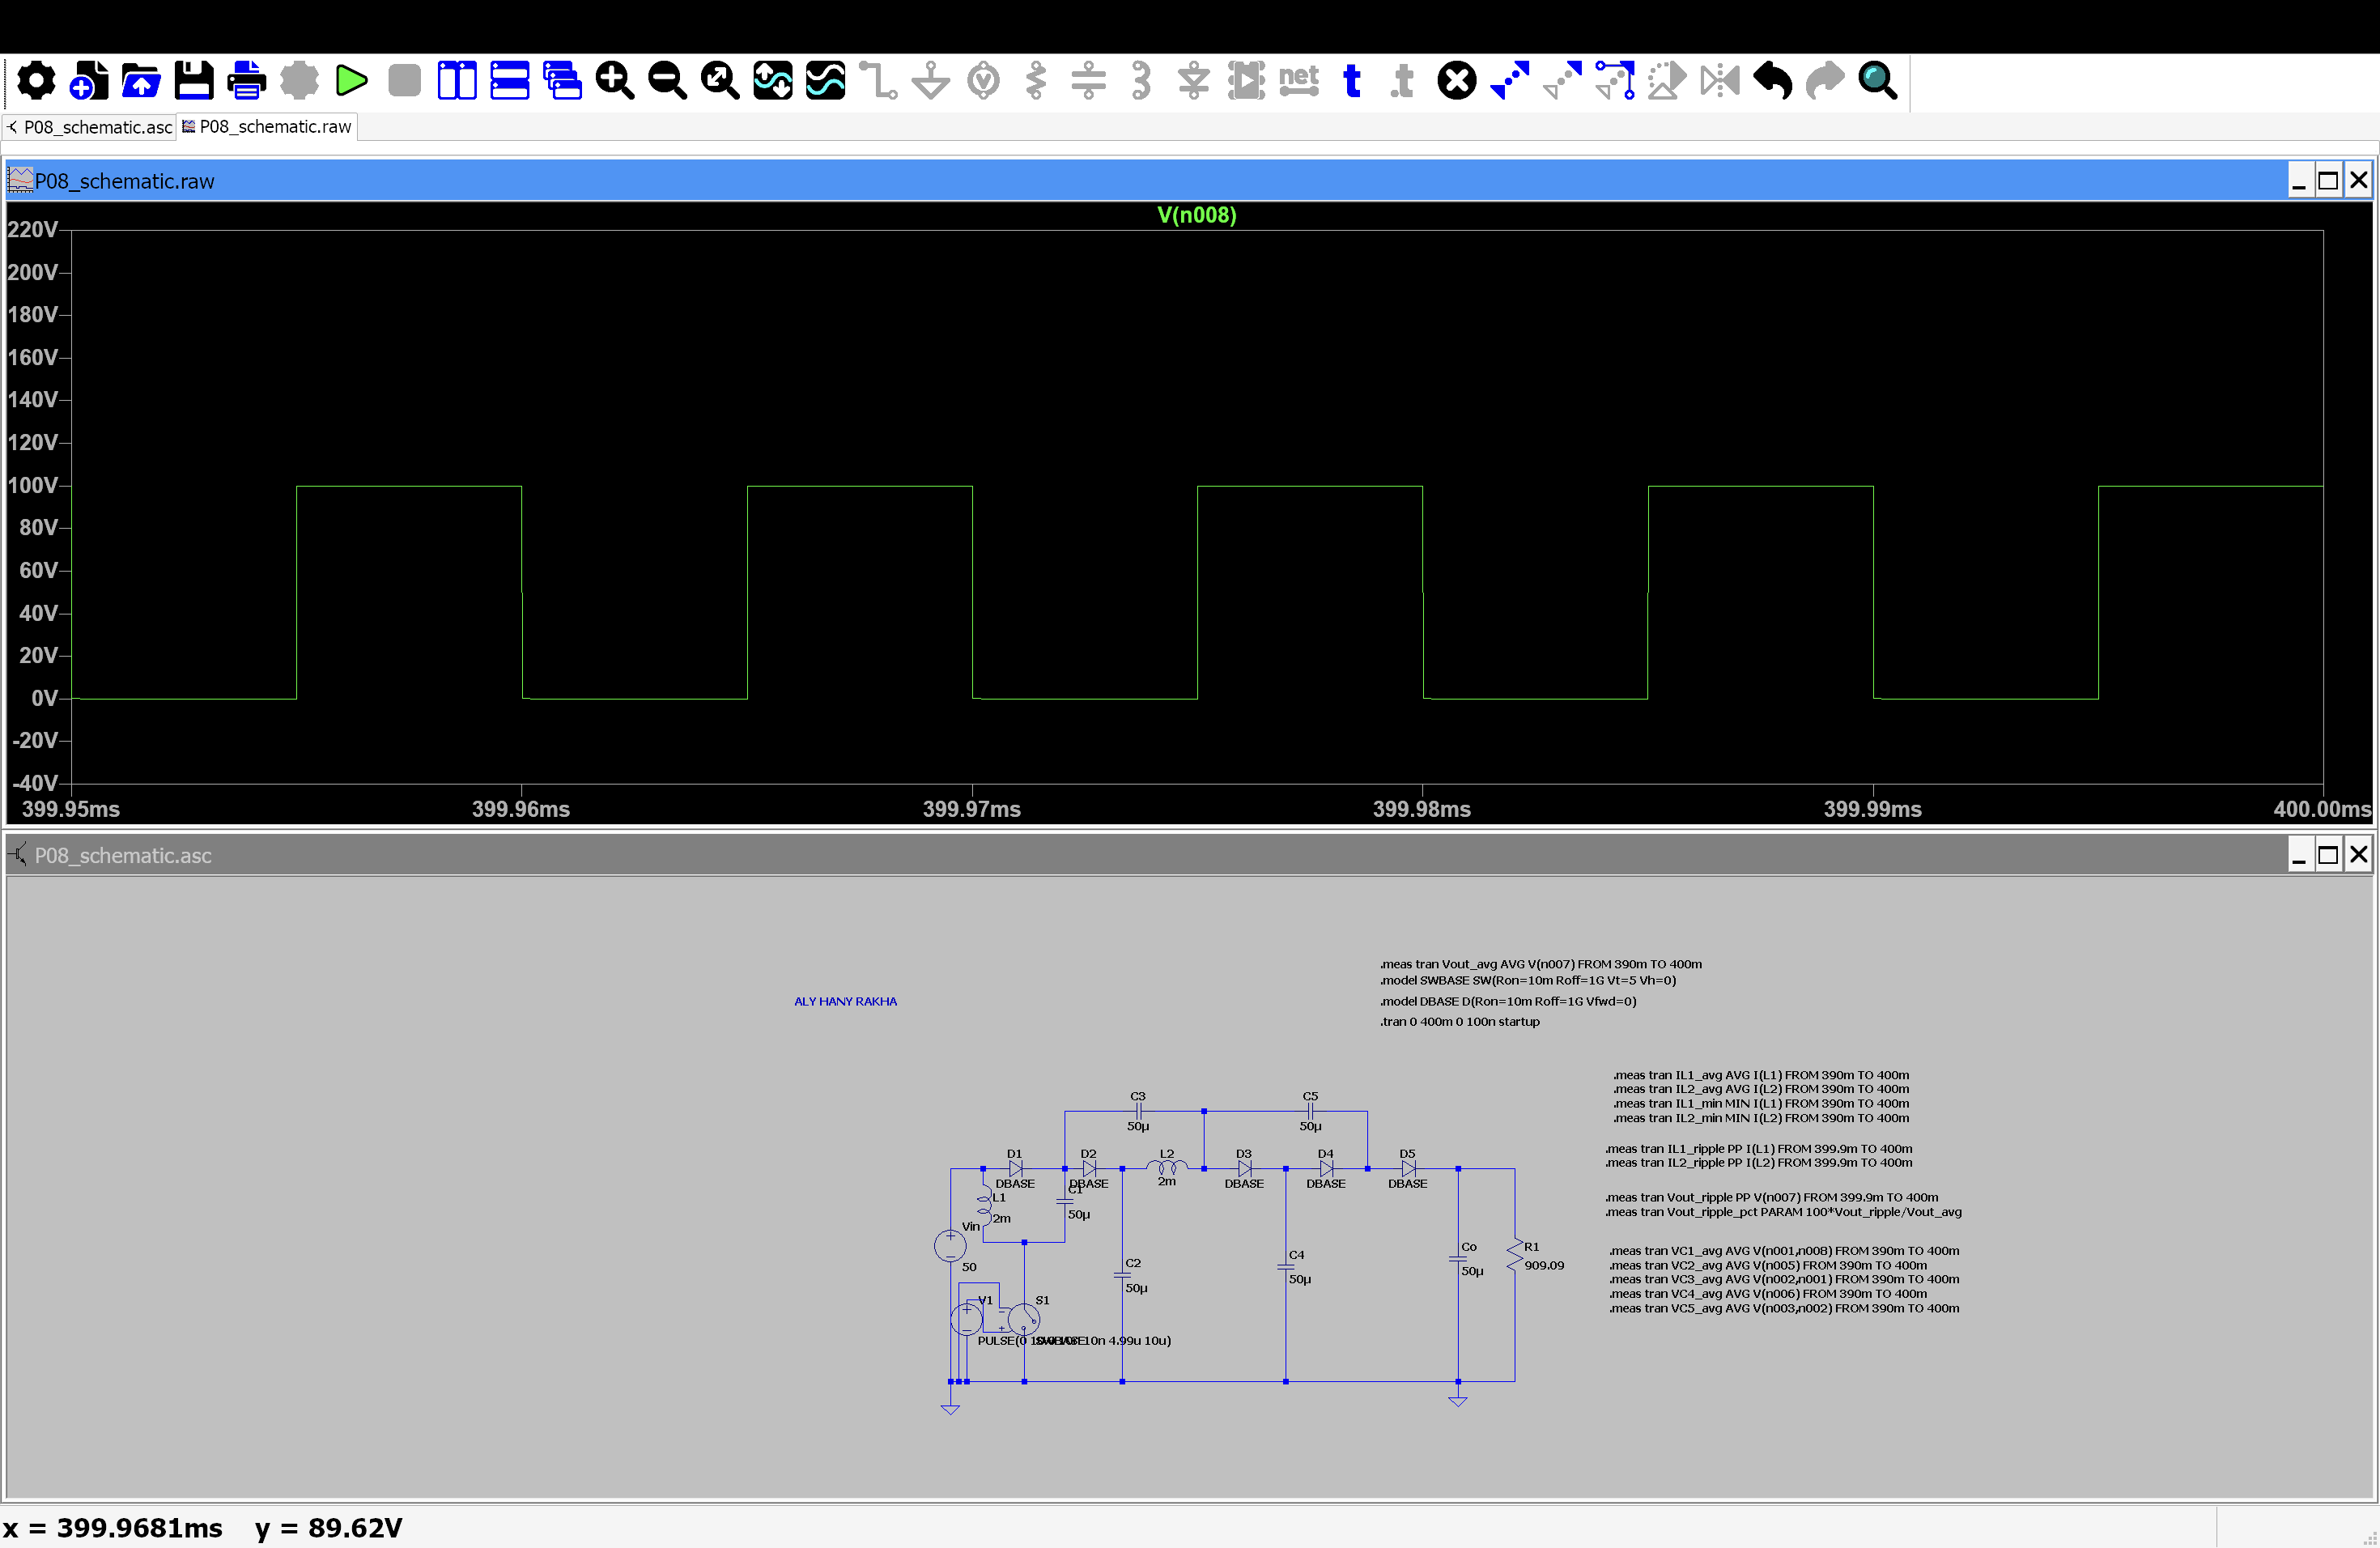
\includegraphics[trim={0bp 444bp 0bp 98bp},clip,width=1\linewidth]{figures/photo18.png}
\caption{Original LTspice switch-voltage waveform over five settled cycles. The voltage alternates between approximately zero and 100 V.}
\end{figure}
These waveforms demonstrate periodic switching and the expected blocking level. They do not establish that a physical converter can tolerate the simulated startup: real inductors may saturate, device ratings may be exceeded, and wiring parasitics may add further overshoot. Those effects were not represented by the near-ideal model.
\clearpage
\section{Effect of duty cycle}\label{sec:duty}
Changing duty cycle provides a stronger check than matching one operating point. The input, inductances, capacitances, load and switching frequency were held constant. Only the pulse width changed.
\begin{table}[H]\centering\caption{Near-ideal duty-cycle comparison. Ripple values are peak-to-peak.}
\begin{tabular}{@{}lrrr@{}}\toprule
Quantity & $D=0.30$ & $D=0.50$ & $D=0.60$ \\\midrule
Predicted output (V) & 214.286 & 300.000 & 375.000 \\\
Simulated output (V) & 213.973 & 299.452 & 374.414 \\\
Output error (\%) & $-0.146$ & $-0.183$ & $-0.156$ \\\
Average $I_{L1}$ (A) & 0.773 & 1.647 & 2.678 \\\
Average $I_{L2}$ (A) & 0.235 & 0.330 & 0.412 \\\
Minimum $I_{L2}$ (A) & 0.198 & 0.266 & 0.335 \\\
$\Delta i_{L1}$ (A) & 0.07489 & 0.12490 & 0.14990 \\\
$\Delta i_{L2}$ (A) & 0.07483 & 0.12473 & 0.14972 \\\
Output ripple (mV) & 16.36 & 33.20 & 51.70 \\\
Steady-state switch maximum (V) & 71.48 & 100.07 & 125.14 \\\
Startup switch maximum (V) & 148.27 & 202.19 & 246.19 \\\bottomrule
\end{tabular}
\end{table}
The original LTspice captures for the 30\% and 60\% duty tests are shown on the following page. The numerical comparison above uses the measurements recorded in their simulation logs.
Increasing the duty cycle raises output voltage and switch stress. Because the load resistance is fixed, output power also rises: approximately 50.4 W, 98.6 W and 154.2 W, using $\overline V_o^2/R$ as a close approximation at small ripple. These are not constant-power comparisons. All three steady-state tests remain in CCM.

The ripple tests also clarify the apparent discrepancy in the paper's Equation (4). At 30\% duty, its printed $L_2$ expression predicts 0.175 A, while the switching-state derivation predicts 0.075 A and the simulation gives 0.07483 A. At 60\%, the printed expression predicts 0.100 A, whereas the derivation predicts 0.150 A and the simulation gives 0.14972 A. These results support the $D$-dependent expression for this circuit and indicate a likely typographical inconsistency in the paper.
\clearpage
\subsection{Original LTspice duty-cycle results}
\begin{figure}[H]\centering
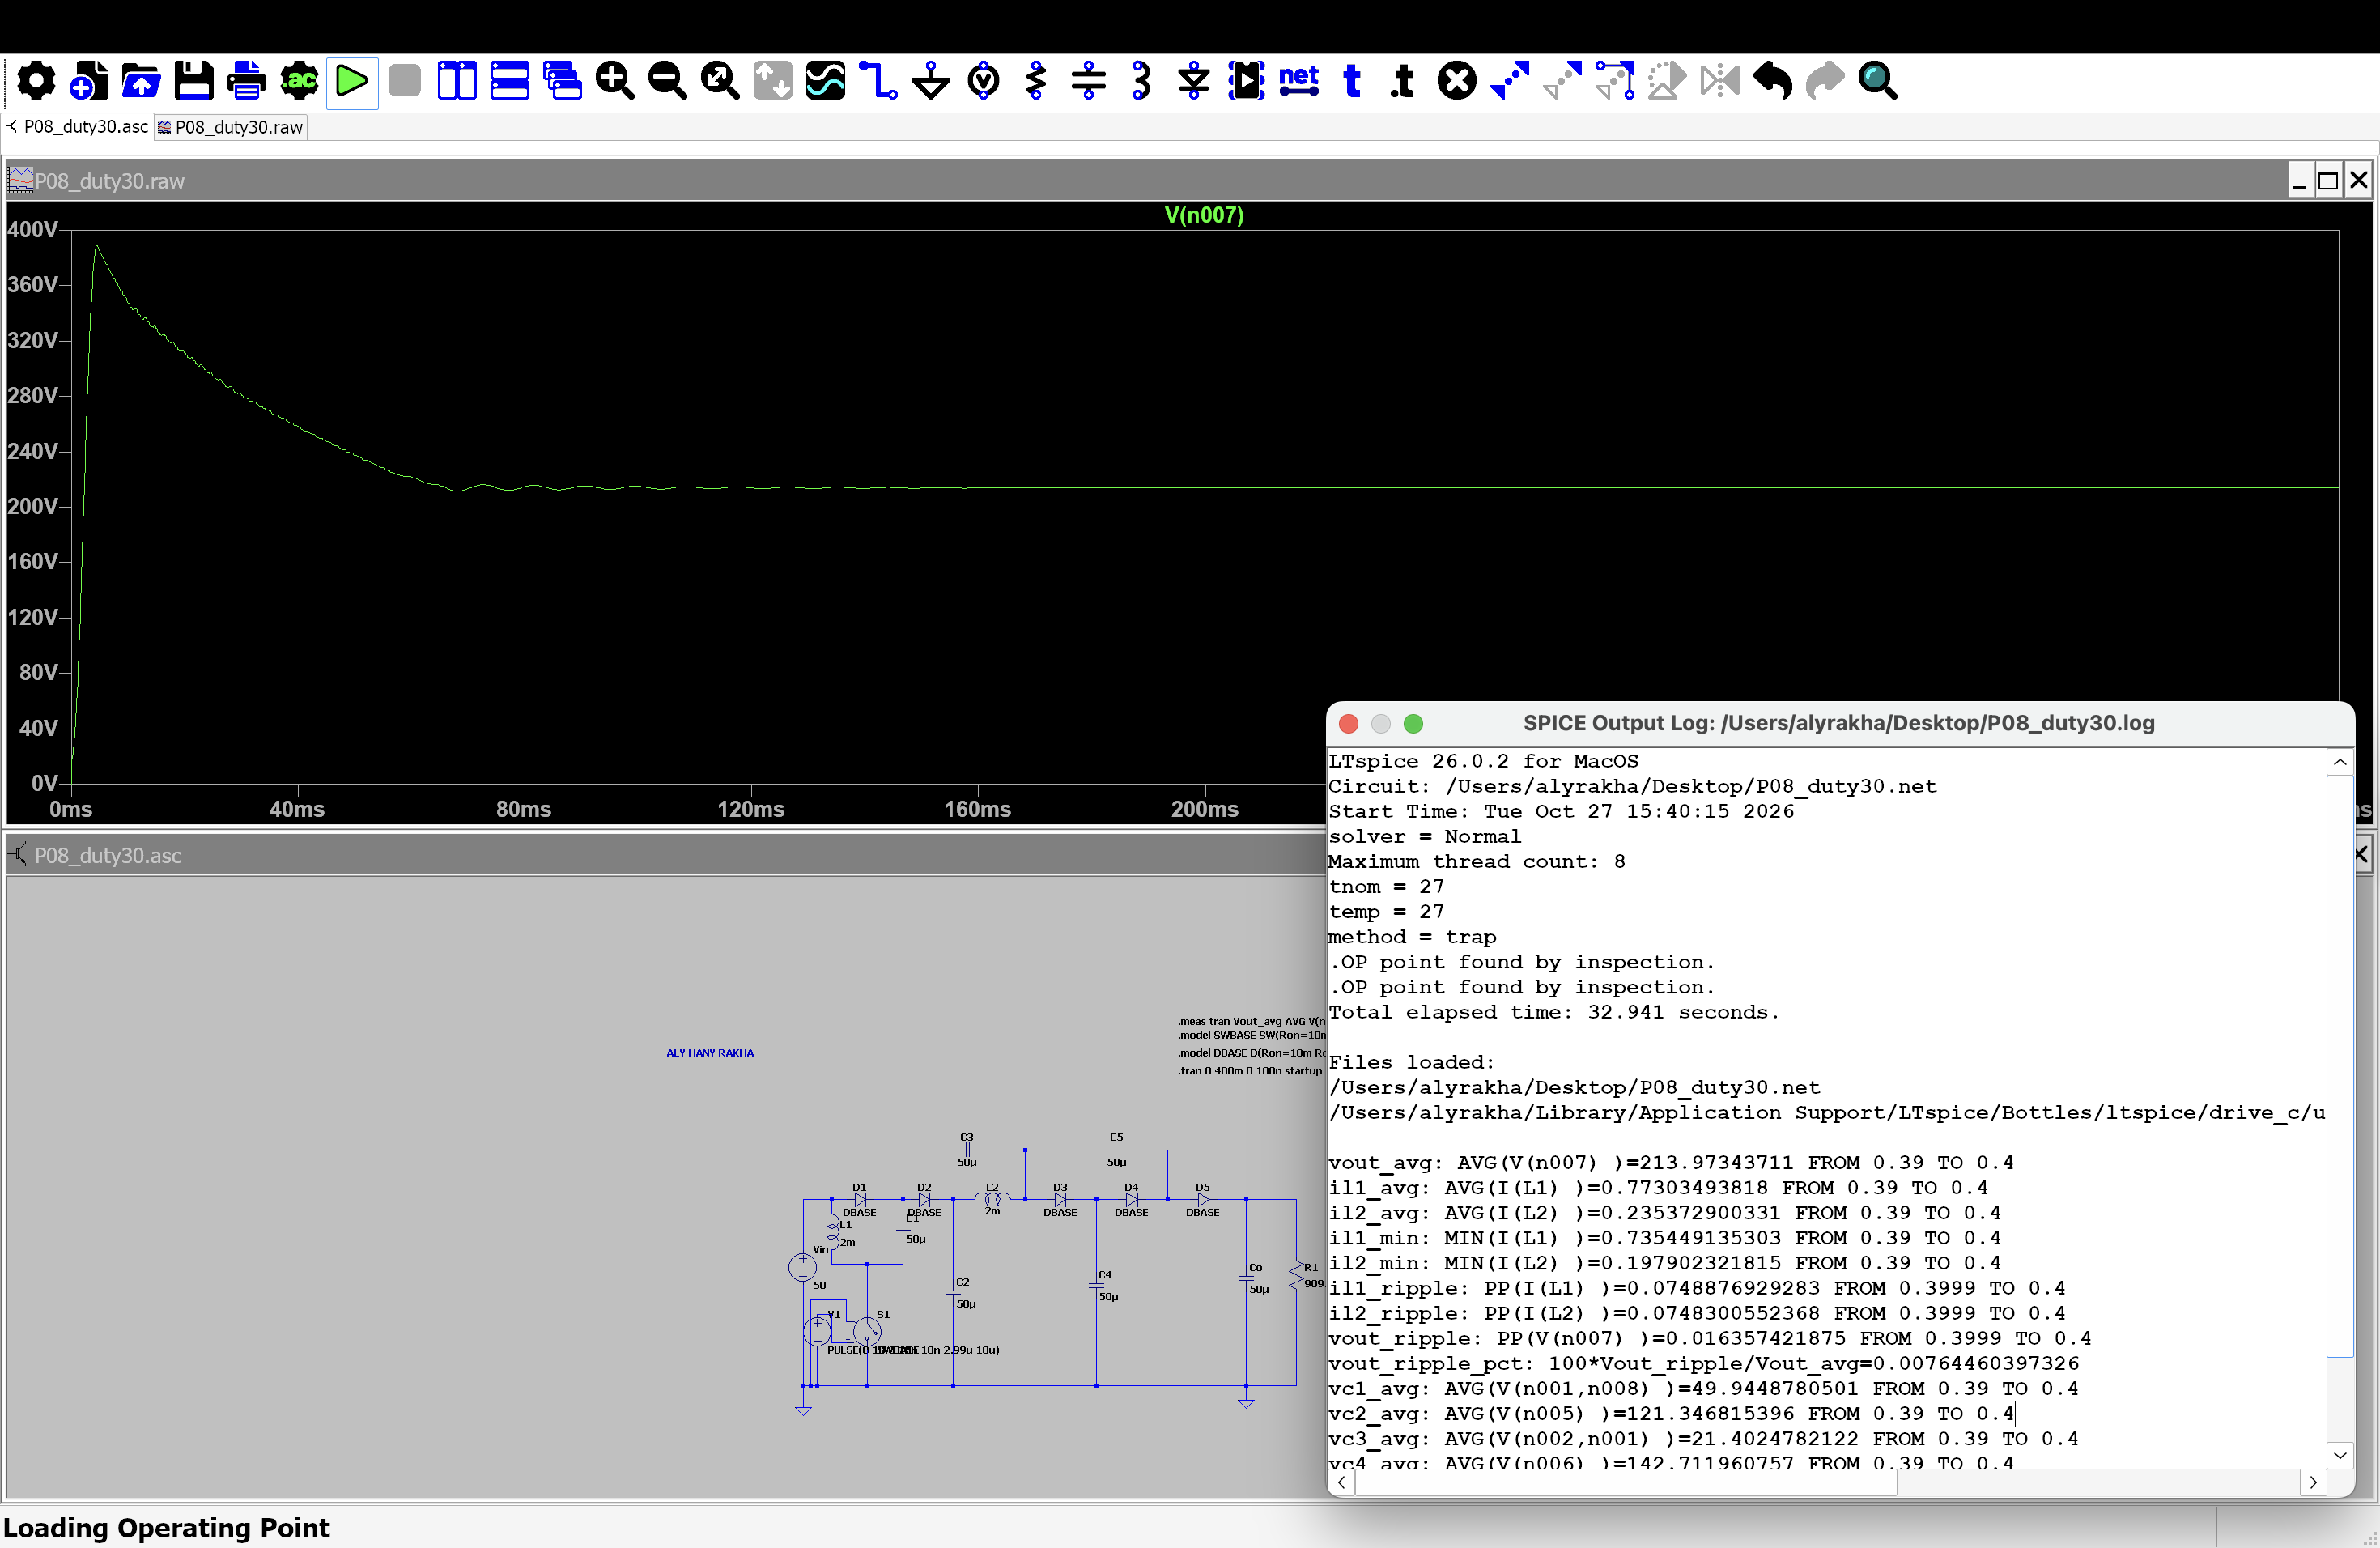
\includegraphics[trim={0bp 444bp 0bp 98bp},clip,width=1\linewidth]{figures/photo19.png}
\caption{Original LTspice capture for 30\% duty: output startup waveform, cropped from the original capture. The numerical measurements are retained in the accompanying logs. The average output is 213.97 V.}
\end{figure}
\begin{figure}[H]\centering
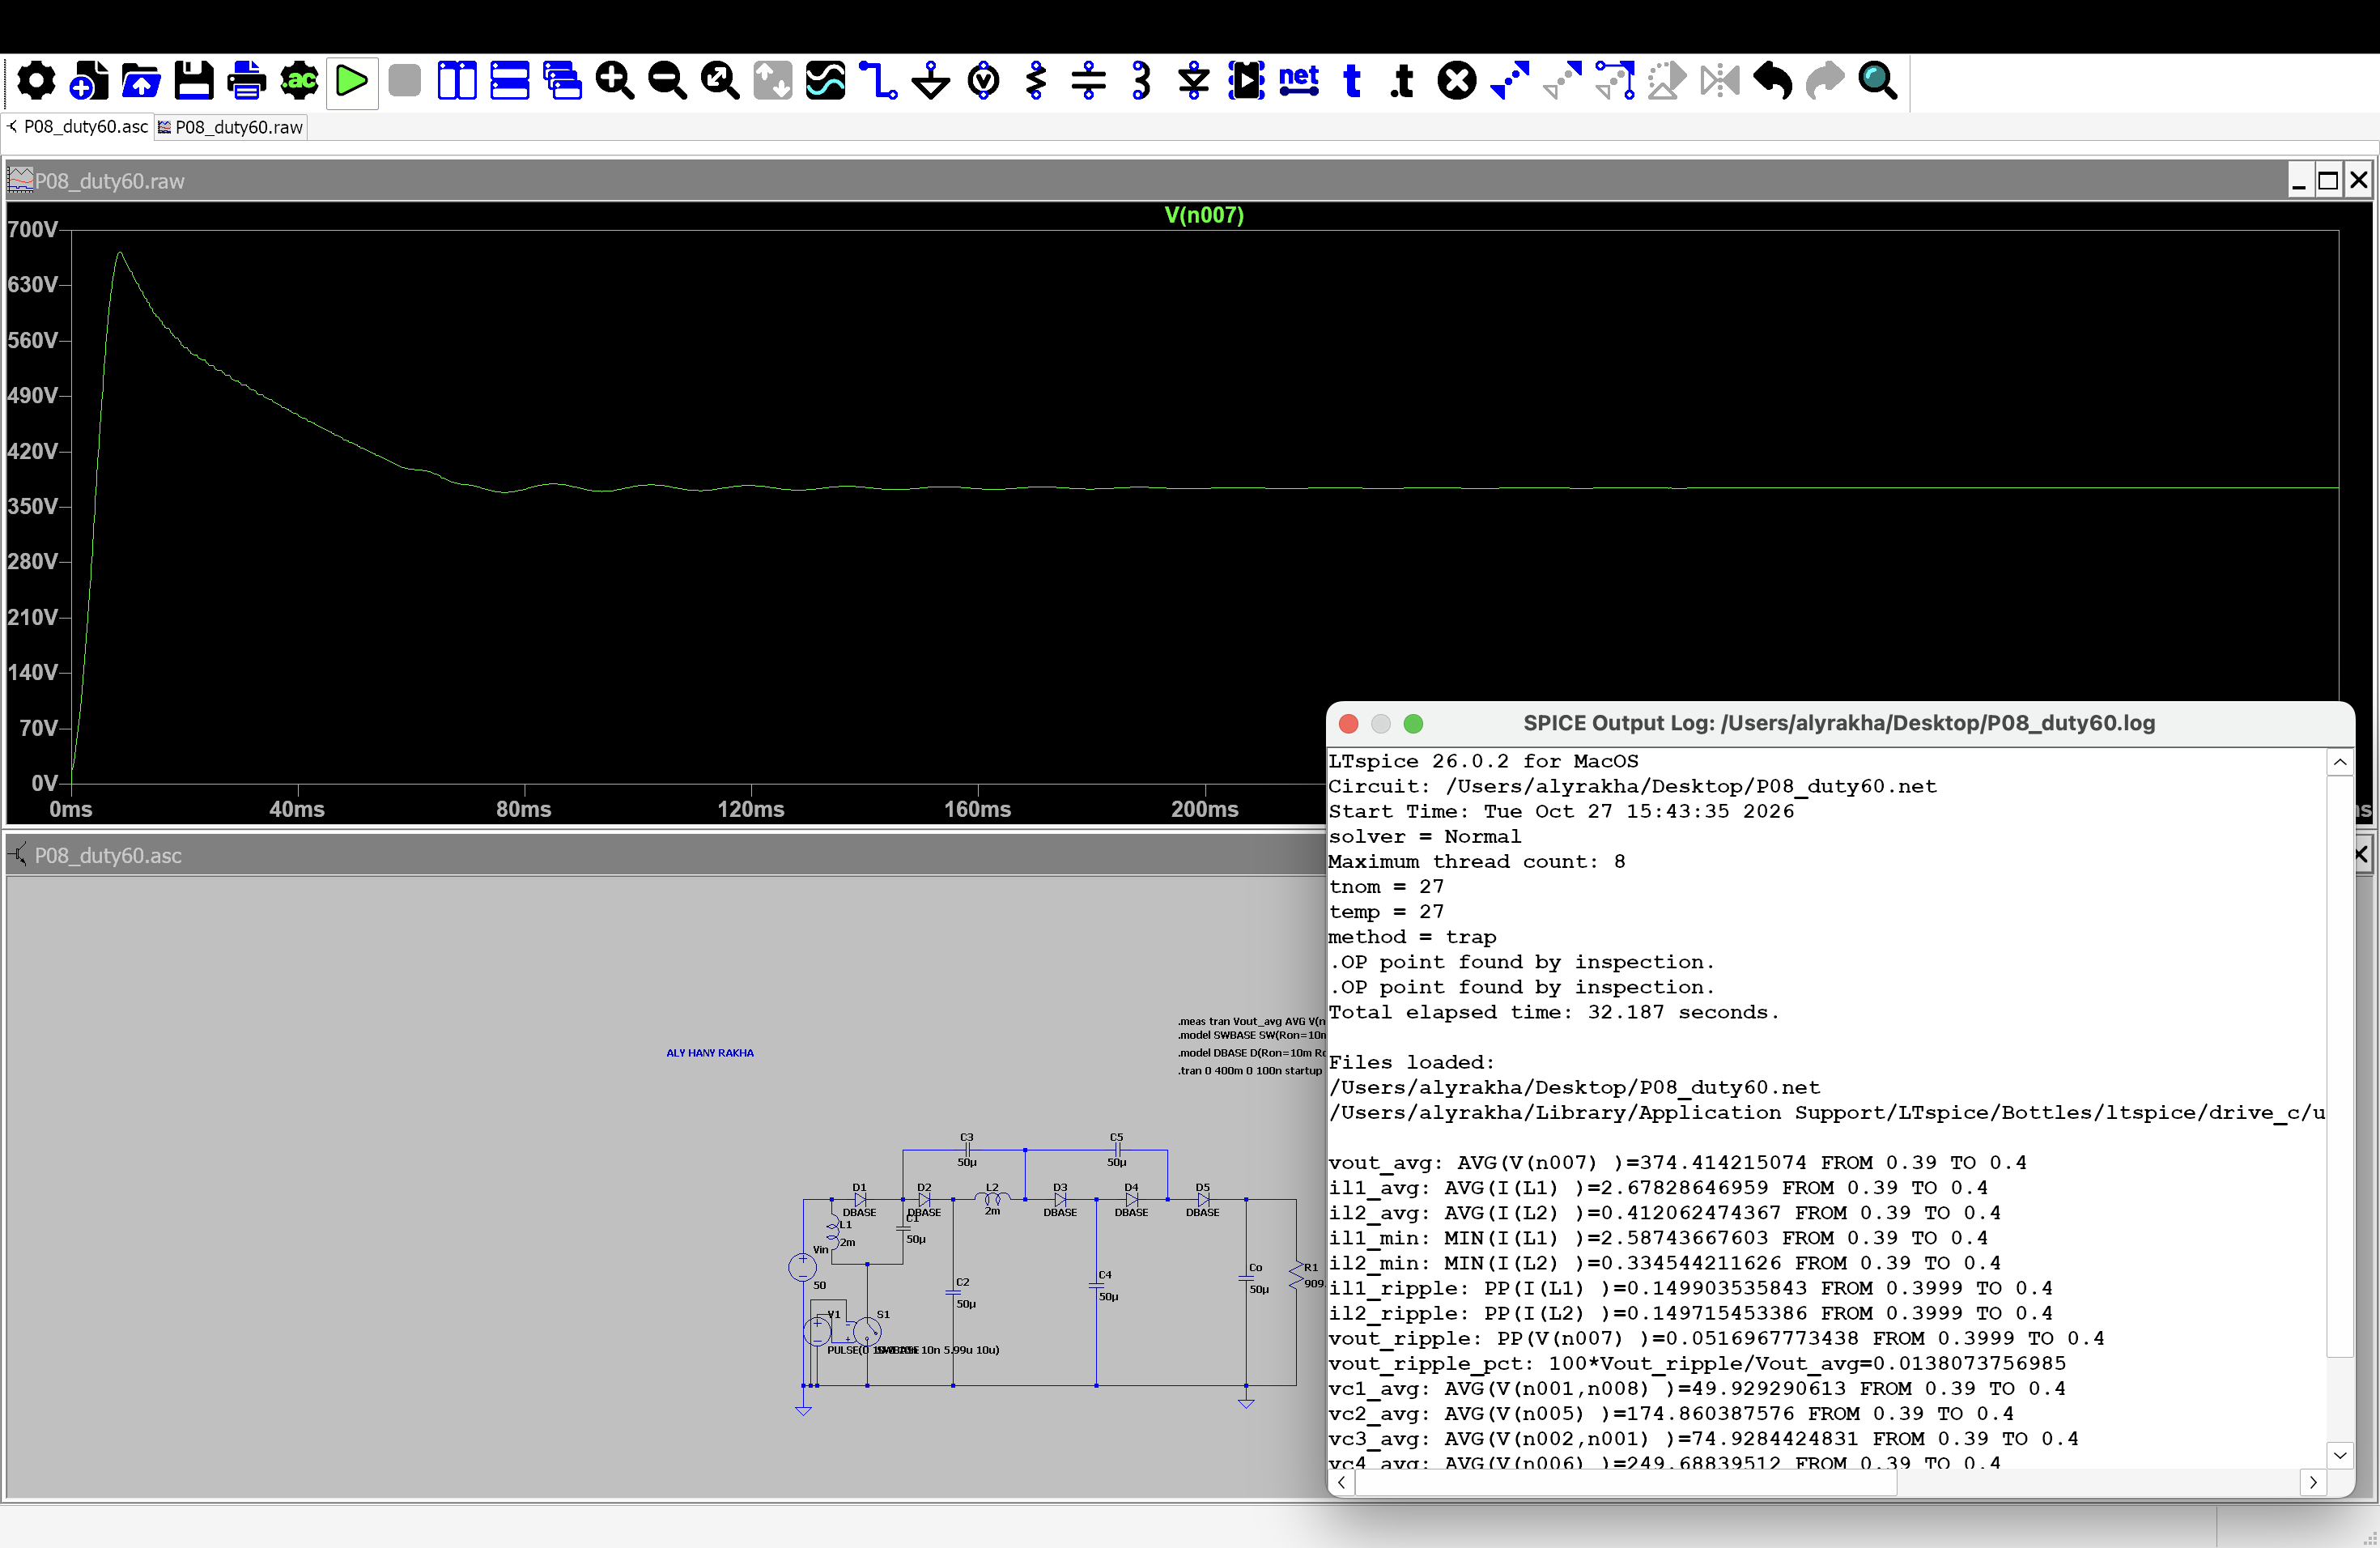
\includegraphics[trim={0bp 444bp 0bp 98bp},clip,width=1\linewidth]{figures/photo20.png}
\caption{Original LTspice capture for 60\% duty: output startup waveform, cropped from the original capture. The numerical measurements are retained in the accompanying logs. The average output is 374.41 V.}
\end{figure}
\clearpage
\section{Conduction losses and MOSFET simulation}\label{sec:loss}
The near-ideal model verifies the topology but cannot represent all practical losses. A second model uses $0.1\unit{\Omega}$ series resistance in each inductor, $0.05\unit{\Omega}$ ESR in every capacitor, $0.05\unit{\Omega}$ switch on-resistance, and a diode model with 0.8 V forward threshold and $0.02\unit{\Omega}$ on-resistance. These are illustrative assumptions.

A third model replaces the voltage-controlled switch with the installed LTspice model of the IPP600N25N3 MOSFET. A $10\unit{\Omega}$ resistor connects the 0--10 V pulse source to its gate, and the source is grounded. This includes the model's gate charging and capacitance effects. The diodes remain simplified conduction models, and the circuit still uses the same assumed inductor and capacitor resistances. It is therefore a more detailed simulation, not an exact recreation of the paper's IRF540/FES8GT prototype.

Power was calculated from instantaneous voltage-current products and then averaged:
\begin{align}
P_{in}&=\left\langle -v_{in}(t)i_{Vin}(t)\right\rangle,&
P_o&=\left\langle \frac{v_o^2(t)}{R}\right\rangle,\\
P_g&=\left\langle-v_g^{source}(t)i_{V1}(t)\right\rangle,&
\eta&=\frac{P_o}{P_{in}+P_g}\times100\%.
\end{align}
The minus signs account for LTspice's current direction into the positive terminal of a voltage source. Gate-source power is included for the MOSFET case. The total simulated loss is $P_{in}+P_g-P_o$. It should not be calculated from $V_{in}I_{L1}$, because $L_1$ does not carry the full source current.
\begin{table}[H]\centering\caption{Recorded loss-model results at approximately 50\% duty.}
\begin{tabular}{@{}lrrr@{}}\toprule
Quantity & Conduction model & MOSFET, 100 ns & MOSFET, 50 ns \\\midrule
Average output (V) & 293.362 & 295.164 & 295.103 \\\
Output ripple (mV) & 54.75 & 84.26 & 79.44 \\\
Main input power (W) & 96.767 & 98.204 & 98.147 \\\
Gate-source power (W) & --- & 0.01963 & 0.01961 \\\
Output power (W) & 94.668 & 95.834 & 95.794 \\\
Total simulated loss (W) & 2.099 & 2.390 & 2.372 \\\
Efficiency (\%) & 97.831 & 97.567 & 97.584 \\\bottomrule
\end{tabular}
\end{table}
The output falls below the near-ideal result when losses are added. The MOSFET model produces a slightly higher output than the fixed-resistance switch model, despite a slightly lower calculated efficiency. This is not contradictory: the MOSFET's effective conduction and switching behavior differs from a fixed $50\unit{m\Omega}$ switch, changing both the output and input power.

The efficiency figures describe these specific models. They exclude unmodeled magnetic core losses, full diode reverse recovery, a practical gate-driver supply, temperature rise and layout parasitics. They cannot be treated as measured hardware efficiencies or as proof of matching the paper's experimental loss distribution.
\clearpage
\section{MOSFET waveforms and numerical checks}
\begin{figure}[H]\centering
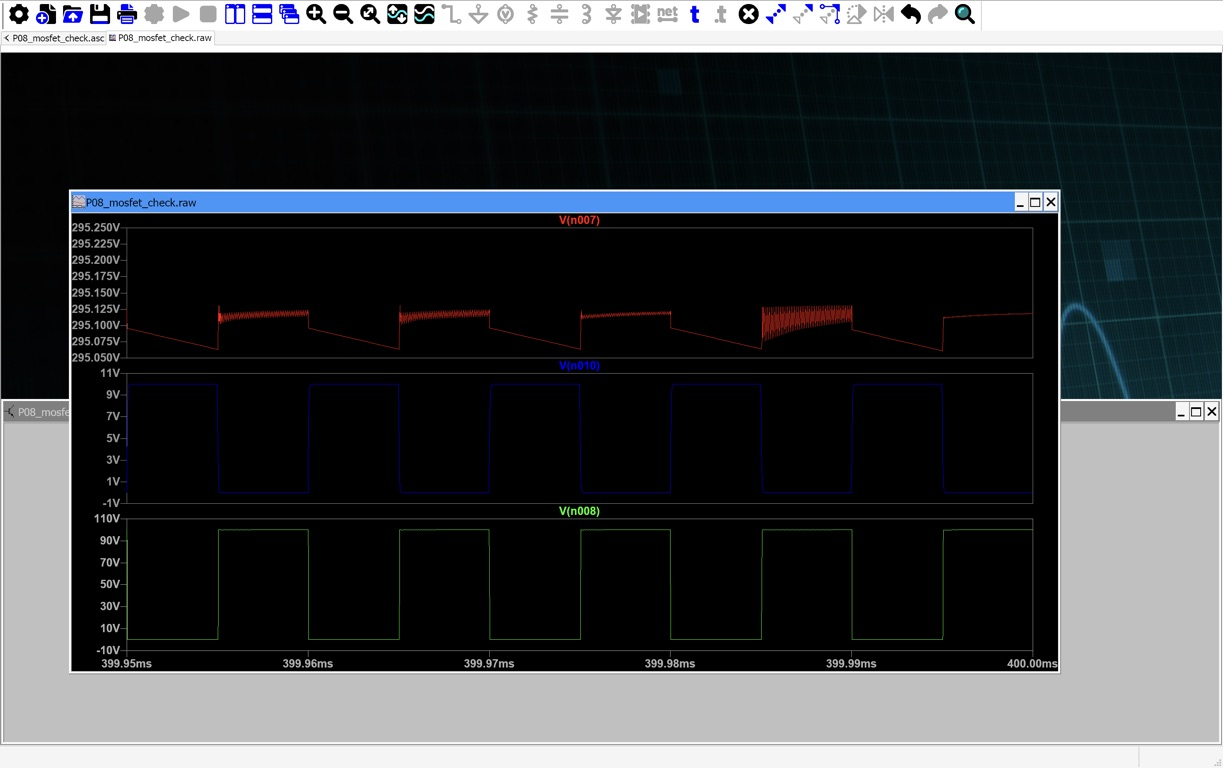
\includegraphics[trim={69bp 94bp 162bp 189bp},clip,width=1\linewidth]{figures/photo30.png}
\caption{Original LTspice screenshot from the final 50 ns MOSFET check, cropped to its waveform window. Top: output voltage, V(n007); middle: gate voltage, V(n010); bottom: drain voltage, V(n008). The time axis spans five settled switching periods.}
\end{figure}
The gate rises to approximately 10 V while the drain falls close to zero. When the gate returns low, the drain rises to approximately 100 V. The output capacitor discharges during the on interval and is replenished during the off interval, giving a small ripple around 295.1 V. Switching edges introduce faster oscillations into the output trace.

The final run uses a maximum timestep of 50 ns instead of 100 ns and disables waveform compression with \texttt{.options plotwinsize=0}. Average output changes by about 0.0617 V, or 0.0209\%, and efficiency changes by 0.0166 percentage points. The average operating point is therefore similar in these two runs. Output ripple changes from 84.26 to 79.44 mV, approximately 5.7\%, showing that a small ripple measurement is more sensitive than the average voltage.

This comparison changes both timestep and compression, so it is not a controlled timestep-convergence study. The solver uses trapezoidal integration, and the visible high-frequency oscillations have not been separated into physical model effects and numerical ringing. A stronger validation would vary timestep alone, compare an alternative integration method, and use measured or manufacturer-supported parasitic models. The present report therefore treats the ripple values as model-dependent simulation results.

For the final MOSFET run, the measured drain maximum is 100.32 V in steady state and 168.67 V during the first 100 ms. The startup value is again materially higher than the steady-state stress. The large startup currents and voltage overshoots would require separate attention before any physical construction.
\clearpage
\section{Comparison with the paper and interpretation}
\subsection{What was reproduced, and what was not}
The closest comparison is with the paper's Table II and the base-converter experimental traces in Figure 12. Both describe the same nominal 50 V input, 50\% duty operating point. The capacitor-voltage levels and inductor-current ramps in the LTspice results agree with that operating principle. The comparison is primarily numerical and qualitative; the paper does not provide raw experimental data for a sample-by-sample waveform comparison.

The simulated startup is a separate observation. It should not be claimed as a reproduction of an experimental startup test, because the paper's reported steady-state waveforms do not establish the same initial conditions. Similarly, the simulated 97.58\% efficiency is not an experimental measurement from the paper.
\begin{table}[H]\centering\caption{Relationship between the paper and this work.}
\begin{tabularx}{\linewidth}{@{}p{.29\linewidth}X@{}}\toprule
Paper topic & Evidence and scope of this report \\\midrule
Triple-converter operation & Both switching states are explained, with voltage-balance derivations and an implemented LTspice circuit. \\
Nominal capacitor voltages and currents & Compared numerically with Table II; inductor waveforms are shown in original LTspice captures. \\
Voltage gain & Tested at 30\%, 50\% and 60\% duty with the same input and resistive load. \\
Nonideal behavior & Explored using assumed conduction losses and an installed MOSFET model; not fitted to the prototype. \\
Quadruple and hextuple extensions & Discussed analytically; not simulated here. \\
Hardware validation & Not performed. Temperature, magnetic saturation and layout-dependent effects remain outside the model. \\\bottomrule
\end{tabularx}
\end{table}
\subsection{How to interpret the loss analysis}
Section III of the paper considers conduction losses in the inductors, switch and diodes, while explicitly ignoring frequency-related losses. Resistive dissipation depends on RMS current, $P_R=I_{rms}^2R$, so average current alone is not enough to calculate the loss in a pulsed branch. A diode also dissipates power through its forward voltage drop. The paper approximates the combined forward-drop loss of the five diodes as $5V_{DF}I_o$.

For example, using the assumed 0.8 V drop and nominal 0.33 A output current gives $5(0.8)(0.33)=1.32\unit{W}$ before adding diode resistance. This explains why diode losses can be significant even when the output voltage is hundreds of volts. It is an estimate, not an independently measured loss breakdown. The report's efficiency calculation instead uses the total source and load powers from the simulation.

The paper's loss plots motivate testing nonideal models, but a single simulated efficiency cannot reproduce their full component-quality or output-power sweeps. The present results establish the direction and approximate size of the changes for the selected assumptions. They do not prove that the converter is always more efficient than competing topologies.
\clearpage
\section{Parts of the paper not implemented in this simulation}
The simulation covers the complete triple-converter power stage, rather than only a disconnected part of it. The main circuits not built in LTspice are the quadruple and hextuple extensions in the paper's Figure 8. This section explains their purpose and operation from the paper, and separates those explanations from results established by my own simulations. Focusing on the triple circuit made it possible to examine its current paths, capacitor voltages, startup and nonideal behavior in detail. The higher-gain variants remain an analytical part of this report.

\subsection{What the additional voltage-lift network does}
The extensions retain one controlled switch and two inductors. Their higher gain comes from rearranging and expanding the diode--capacitor network, rather than adding independently controlled boost stages. An inductor stores energy in its magnetic field, while a lift capacitor stores charge and maintains a voltage between two circuit nodes. The diodes determine which charging and transfer paths are available as the switch changes state.

The important point is that a lift capacitor need not have its negative terminal at ground. Once charged, it can connect two nodes at different DC levels. Its stored voltage then contributes to a higher node voltage during the appropriate transfer interval. The diode orientation prevents an unwanted reverse discharge through the same path. Repeating this process establishes several capacitor voltage levels whose contributions increase the output. The output capacitor has a different role: it supplies the load between transfer intervals and limits output ripple. The capacitors do not generate energy; the input source supplies the energy delivered to the load and dissipated in losses.

\subsection{Quadruple converter: the first extension}
Figure 8(a) of the paper adds diode--capacitor lift paths to the base arrangement. Its horizontal capacitor branches connect intermediate nodes, while the vertical capacitor branches maintain the intermediate voltage levels relative to the return. These branches allow one more lift contribution than the triple topology. The main switch still alternates between an energy-storage interval and an energy-transfer interval, but the extra diodes establish additional charging paths within those intervals. The exact conducting-diode list must be worked out for this extended schematic; the triple converter's diode labels and state list cannot simply be copied into it.

The paper gives the ideal continuous-conduction gain as
\begin{equation}
M_{quad}=\frac{V_o}{V_{in}}=\frac{4}{1-D}.
\end{equation}
For $V_{in}=50\unit{V}$ and $D=0.5$, the prediction is $V_o=400\unit{V}$, compared with 300 V for the triple converter. At the same duty ratio, the ideal output is therefore $4/3$ times the triple output. This is the meaning of the extra lift contribution; it does not mean that the output is always exactly four times the input.

\subsection{Hextuple converter: the second extension}
Figure 8(b) expands the lift network further, including additional bridging diode paths and capacitor branches. These paths establish more stored voltage contributions while retaining the same number of inductors and controlled switches. The topology is consequently more involved to wire and verify, even though its gate-drive arrangement still uses a single controlled switch.
\begin{equation}
M_{hex}=\frac{V_o}{V_{in}}=\frac{6}{1-D}.
\end{equation}
At the same 50 V input and 50\% duty, the predicted output is 600 V: twice the triple converter's ideal output. The paper reports 400 V and 600 V for the two extensions in its experimental gain demonstration, Figure 13. These are the authors' results, not additional LTspice runs performed for this report \cite{paper}.
\subsection{What would need to be checked for the extensions}
A higher voltage gain does not imply a free increase in output power. With the same $909.09\unit{\Omega}$ load used here, ideal outputs of 400 V and 600 V would imply approximately 176 W and 396 W, respectively, from $P_o=V_o^2/R$. Those would not be comparable 100 W tests. To compare all three topologies at 100 W, the ideal load values would instead be approximately $900\unit{\Omega}$, $1600\unit{\Omega}$ and $3600\unit{\Omega}$ for 300 V, 400 V and 600 V. These are calculated test conditions, not simulated results.

A meaningful replication would first redraw each Figure 8 circuit and identify its charging paths in both switch states. Each capacitor voltage should then be checked using charge balance, and each inductor using volt-second balance. A transient simulation would need to confirm capacitor polarity, settled gain, positive inductor-current minima, output ripple and startup stress. The base circuit's capacitor voltages and semiconductor ratings cannot be assumed to apply unchanged to the extensions. More diodes and capacitors also introduce additional conduction losses, charging currents and stored energy. This is why the gain equations alone are not enough to select components or establish efficiency.

\subsection{Discontinuous conduction and operating-region analysis}
The paper also discusses the boundary between continuous and discontinuous conduction in Figure 4. The steady-state measurements in this report remain in CCM: both inductor currents stay above zero in the measured intervals. I did not carry out a light-load sweep to reproduce the boundary or establish the behavior in DCM.

At a sufficiently light load, or with a sufficiently small inductance, the current ripple can become comparable to the average current. If an inductor current reaches zero and stays there for part of the period, the two-state CCM description is no longer sufficient. The conducting paths and time intervals must be reconsidered, and the CCM gain cannot be assumed to remain valid. For an approximately triangular current, $I_{L,avg}-\Delta I_{L,pp}/2=0$ is a useful first indication of the boundary, but each inductor must be checked separately. A future load sweep would test where the minimum currents reach zero and compare that transition with the paper's operating-region analysis. Brief current reversals during startup are not, by themselves, proof of a settled DCM operating point.

\subsection{Loss sweeps, hardware and application-level functions}
Figures 5--7 examine nonideal gain and efficiency as power and component losses change. My loss and MOSFET models examine selected operating points; they do not reproduce those complete sweeps. Recreating them would require varying the load and parasitic resistances systematically, measuring input and output power after settling, and maintaining the same assumptions as the paper. The paper's conduction-loss analysis omits frequency-related losses, whereas a MOSFET transient model can include some switching effects. These two approaches therefore require careful interpretation before their efficiency values are compared.

The prototype in Figure 11 was not built here. The simulation does not establish magnetic saturation, temperature rise, layout parasitics or the performance of the paper's particular hardware. Likewise, the title's renewable-energy application is a motivation for the step-up stage: neither this simulation nor the gain equations constitute a complete photovoltaic system. My circuit uses a fixed DC source and open-loop gate pulses. A photovoltaic model, maximum-power-point tracking, output-voltage feedback and a grid interface were not implemented; they are possible system additions, rather than missing blocks of the simulated triple power stage. A regulated system would measure the output and adjust duty when input voltage or load changes, instead of keeping the pulse width fixed.

For context, an ideal ordinary boost converter would need $D=1-50/300=0.833$ to obtain 300 V from 50 V, while the triple topology reaches that ratio at $D=0.5$. This explains the attraction of the lift network. A fair overall comparison would also consider efficiency, device count, startup behavior and cost at equal power. All three proposed circuits share an input and output ground, so their voltage gain does not provide galvanic isolation.

\subsection{Main lessons from the replication}
The most useful part of the comparison was linking each waveform back to a circuit state. A high gate voltage turns the MOSFET on and pulls its drain low; the inductors charge while the output capacitor supplies the load. During the off interval, the drain voltage rises and the stored energy is transferred through the diode network. That explanation makes the plots more meaningful than simply reporting a final output near 300 V.

The investigation also showed why steady-state and startup results must be kept separate. The near-ideal switch voltage is about 100 V after settling but exceeds 200 V during startup. Likewise, positive settled inductor currents confirm CCM only for the interval measured. The ideal formulas should be used with their assumptions, rather than applied automatically to the whole transient.

Finally, the disagreement between the paper's printed $L_2$ ripple expression and its switching-state equations was checked using two additional duty ratios. This is a stronger basis for discussing the apparent error than assuming that every printed equation must be correct, or rejecting it based on one plot. A further improvement would be to vary timestep and integration method independently before assigning physical meaning to the small high-frequency oscillations.
\clearpage
\section{Conclusions}
The simulation reproduces the main steady-state behavior of the triple voltage-lift modified Luo converter. At the reference operating point, the output is 299.45 V compared with the ideal 300 V prediction. The five intermediate capacitor voltages and the average inductor currents also agree closely with the analysis. Positive minimum inductor currents establish CCM during the measured steady-state intervals.

The duty-cycle tests are particularly useful: they confirm the voltage-gain trend over three operating points and distinguish two conflicting expressions for the second inductor ripple. The simulated ripple agrees with the expression obtained directly from the switching-state equations, suggesting that the paper's printed $(1-D)$ factor is inconsistent with those equations away from 50\% duty.

Introducing losses reduces the output voltage and changes the ripple. The final MOSFET model produces 295.10 V with 95.79 W delivered to the load and 97.58\% simulated efficiency including gate-source power. These results show how the chosen nonidealities affect the converter, but they do not establish the performance of the paper's physical prototype.

The main practical lesson is that steady-state gain is only one part of understanding the circuit. Capacitor polarity, current paths, startup stress and numerical resolution all matter. A useful next stage would be a controlled numerical convergence study followed by more complete diode, magnetic and thermal models. A hardware implementation would additionally require startup control and device-rating checks based on transients as well as steady state.
\begin{thebibliography}{9}
\bibitem{paper} H. Gholizadeh, M. Dehghan, G. B. Gharehpetian and A. Yazdani, ``Triple, Quadruple, and Hextuple Voltage-Lift Modified Luo Converters Suitable for Renewable Applications,'' \emph{IECON 2024 -- 50th Annual Conference of the IEEE Industrial Electronics Society}, 2024. DOI: \href{https://doi.org/10.1109/IECON55916.2024.10905089}{10.1109/IECON55916.2024.10905089}.
\bibitem{ltspice} Analog Devices, \emph{LTspice 26.0.2 for macOS}, installed component models and simulation output. Simulations recorded on 27 October 2026. Model parameters and measurement definitions are included in the accompanying circuit files.
\end{thebibliography}
\clearpage
\appendix
\section{Reproducibility and simulation files}
The repository contains the named schematics, recorded netlists and logs, and available plot settings. The MOSFET uses the installed LTspice library. The large binary waveform files are omitted from the repository; the schematics can regenerate waveforms in LTspice. The original data and screenshots were retained separately.

{\small\begin{tabularx}{\linewidth}{@{}p{.49\linewidth}X@{}}\toprule
Schematic & Purpose \\\midrule
\texttt{P08\_baseline50\_recovered.asc} & Near-ideal 50\% reference circuit. Recovered copy associated with the baseline results. \\\
\texttt{P08\_duty30.asc} & Near-ideal 30\% duty test. \\\
\texttt{P08\_duty60.asc} & Near-ideal 60\% duty test. \\\
\texttt{P08\_loss\_model.asc} & Simplified conduction-loss model at 50\% duty. \\\
\texttt{P08\_mosfet\_model.asc} & MOSFET substitution, 100 ns maximum timestep. \\\
\texttt{P08\_mosfet\_check.asc} & Final MOSFET check, 50 ns and no compression. \\\bottomrule
\end{tabularx}}

The archived 30\% and 60\% schematics contained stale pulse widths. The repository copies use \texttt{2.99u} and \texttt{5.99u}, respectively, consistent with their recorded netlists and logs. The results in this report come from those recorded runs; these packaging corrections are not presented as new simulations. The baseline log and netlist retain the original \texttt{P08\_schematic} filename. Every submitted schematic contains the author's name.

Representative measurements are shown below. They should be entered as SPICE directives, not as component values. Averages are taken over the last 10 ms; ripple is measured over the last $100\unit{\mu s}$.
\begin{verbatim}
.meas tran Vout_avg AVG V(n007) FROM 390m TO 400m
.meas tran IL1_min MIN I(L1) FROM 390m TO 400m
.meas tran IL2_min MIN I(L2) FROM 390m TO 400m
.meas tran IL1_ripple PP I(L1) FROM 399.9m TO 400m
.meas tran IL2_ripple PP I(L2) FROM 399.9m TO 400m
.meas tran Vout_ripple PP V(n007) FROM 399.9m TO 400m
.meas tran Pin AVG (-V(n004)*I(Vin)) FROM 390m TO 400m
.meas tran Pout AVG (V(n007)*V(n007)/909.09) FROM 390m TO 400m
.meas tran Pgate AVG (-V(n009)*I(V1)) FROM 390m TO 400m
.meas tran Pin_total PARAM Pin+Pgate
.meas tran Efficiency_total_pct PARAM 100*Pout/Pin_total
\end{verbatim}
The gate-power expression applies to the MOSFET schematics, where \texttt{n009} is the drive-source node. A sign or node error can produce a plausible-looking but incorrect efficiency, so source polarity and node labels must be checked before reusing these expressions in a modified circuit.

Selected original LTspice captures are included in the repository. Only completed simulation results are used as quantitative evidence in this report. All waveform figures in this report are original LTspice screenshots. Where the surrounding desktop or schematic is omitted, only the displayed crop has changed; the plotted traces, labels and axes have not been redrawn. The source screenshots used here are retained in report/figures.
\end{document}
